\documentclass[11pt]{article}


%\newcommand{\citep}[1]{\cite{Graham-#1}}
%\newcommand{\citet}[1]{\cite{Graham-#1}}

\newcommand{\R}{\mathbf R}
\newcommand{\Z}{\mathbf Z}
\newcommand{\cin}{C_{\text{in}}}
\newcommand{\cout}{C_{\text{out}}}
\newcommand{\wb}{\mathbf W}
\newcommand{\xb}{\mathbf x}
\newcommand{\yb}{\mathbf y}
\newcommand{\calA}{\mathcal{A}}
\newcommand{\bz}{\mathbf{z}}
\newcommand{\bv}{\mathbf{v}}
\newcommand{\bx}{\mathbf{x}}
\newcommand{\ba}{\mathbf{a}}
\newcommand{\calZ}{\mathcaL{Z}}
\newcommand{\SecInd}{{\sc SecInd}\xspace}
\newcommand{\SecAgg}{{\sc SecAgg}\xspace}
\newcommand{\FedAvg}{{\sc FedAvg}\xspace}
\newcommand{\SGD}{{\sc SGD}\xspace}

\def\ie{\textit{i.e.,}\@\xspace}
\def\eg{\textit{e.g.,}\@\xspace}

\newcommand{\pierre}[1]{{\color{purple}Pierre: #1}}
\newcommand{\sayan}[1]{{\color{red}Sayan: #1}}
\newcommand{\karthik}[1]{{\color{blue}Karthik: #1}}
\newcommand{\graham}[1]{{\color{green}Graham: #1}}
\newcommand{\ilya}[1]{{\color{red}Ilya: #1}}
\newcommand{\ashkan}[1]{{\color{blue}Ashkan: #1}}
\newcommand{\dzmitry}[1]{{\color{purple}Dzmitry: #1}}
\newcommand{\modif}[1]{{\color{black}#1}}

\title{Reconciling Security and Communication Efficiency in Federated Learning}
% Communication Efficient and Secure Federated Learning
% Unifying Secure Federated Learning and Communication Efficiency
% The Missing Bit for Practical Efficient Communication in Federated Learning
% Enabling Federated Learning with Communication Efficiency


% The \author macro works with any number of authors. There are two commands
% used to separate the names and addresses of multiple authors: \And and \AND.
%
% Using \And between authors leaves it to LaTeX to determine where to break the
% lines. Using \AND forces a line break at that point. So, if LaTeX puts 3 of 4
% authors names on the first line, and the last on the second line, try using
% \AND instead of \And before the third author name.


\author{
Karthik Prasad\thanks{Equal contribution. Correspondence to \texttt{pstock@fb.com}.} $^{~\dagger}$~~ Sayan Ghosh\footnotemark[1]$^{~~\dagger}$~~ Graham Cormode$^\dagger$~~ \\ {Ilya Mironov$^\dagger$~~ Ashkan Yousefpour$^\dagger$~~ Pierre Stock$^\dagger$} \\ $^\dagger$Meta AI
%   David S.~Hippocampus\thanks{Use footnote for providing further information
%     about author (webpage, alternative address)---\emph{not} for acknowledging
%     funding agencies.} \\
%   Department of Computer Science\\
%   Cranberry-Lemon University\\
%   Pittsburgh, PA 15213 \\
%   \texttt{hippo@cs.cranberry-lemon.edu} \\
  % examples of more authors
  % \And
  % Coauthor \\
  % Affiliation \\
  % Address \\
  % \texttt{email} \\
  % \AND
  % Coauthor \\
  % Affiliation \\
  % Address \\
  % \texttt{email} \\
  % \And
  % Coauthor \\
  % Affiliation \\
  % Address \\
  % \texttt{email} \\
  % \And
  % Coauthor \\
  % Affiliation \\
  % Address \\
  % \texttt{email} \\
}

\begin{document}
\maketitle
\begin{abstract}
Cross-device Federated Learning is an increasingly popular machine learning setting to train a model by leveraging
a large population of client devices with high privacy and security guarantees.
However,
communication efficiency remains a major bottleneck when scaling federated learning to production environments, particularly due to bandwidth constraints during uplink communication.
In this paper, we formalize and address the problem of compressing client-to-server model updates
under the Secure Aggregation primitive, a core component of Federated Learning pipelines that allows the server to aggregate the client updates without accessing them individually.
In particular, we adapt standard scalar quantization and pruning methods
to Secure Aggregation and propose Secure Indexing, a variant of Secure Aggregation that supports quantization for extreme compression.
We establish state-of-the-art results on LEAF benchmarks in a secure Federated Learning setup with up to 40$\times$ compression in uplink communication
with no meaningful loss in utility compared to uncompressed baselines.
% compared to a.
% \karthik{\st{with less than one bit per weight on the LEAF benchmark and no significant loss in utility.}}
% \karthik{I have edited the abstract a bit, please check history to review my changes}
\end{abstract}

% this must go after the closing bracket ] following \twocolumn[ ...
% This command actually creates the footnote in the first column
% listing the affiliations and the copyright notice.
% The command takes one argument, which is text to display at the start of the footnote.
% The \mlsysEqualContribution command is standard text for equal contribution.
% Remove it (just {}) if you do not need this facility.

\section{Introduction}
\label{sec:intro}

Federated Learning (FL) is a distributed machine learning (ML) paradigm that trains a model across a number of participating entities holding local data samples.
% , without exchanging them.
In this work, we focus on \emph{cross-device} FL that harnesses a large number (up to hundreds of millions) of edge devices with disparate characteristics such as availability, compute, memory, or connectivity
resources~\cite{Graham-kairouz2019advances}. %that harnesses potential
% Current applications of FL are designed to scale up to client populations of hundreds of millions or even billions.
Two challenges to the success of cross-device FL are privacy and scalability.
FL was originally motivated for improving privacy since data points remain on client devices.
% and only small model updates were shared to a co-ordinating server.
However, as with other forms of ML, information about training data can be extracted via membership inference or reconstruction attacks on a trained model \cite{Graham-carlini2021membership,Graham-carlini2020extracting}, or leaked through local updates~\cite{Graham-MelisSCS19,Graham-geiping2020inverting}.
Consequently, Secure Aggregation (\SecAgg) protocols were introduced to prevent the server from directly observing individual client updates, which is a major vector for information leakage~\cite{Graham-bonavitz2019federated,Graham-huba2021papaya}.
Additional mitigations such as  Differential Privacy (DP) may be required to offer further protection
against attacks~\cite{Graham-dwork2006calibrating,Graham-abadi2016deep}, as discussed in Section~\ref{sec:discussion}.
% , as discussed in Section~\ref{sec:discussion}.
%As an additional layer of protection against statistical inference attacks, SecAgg is usually paired with Differential Privacy (DP) \cite{Graham-dwork2006calibrating}. To realize the full promise of FL as a privacy-enhancing technology, we need both SecAgg and Differential Privacy.

Ensuring scalability to populations of heterogeneous clients is the second challenge for FL.
% There are many aspects for FL scalability, such as ensuring that model updates can be calculated efficiently
% by devices with various capabilities and intermittent availability~\cite{Graham-bonavitz2019federated}.
% Here, we focus on the communication bottleneck as the primary concern.
Indeed, wall-clock training times are highly correlated with increasing model and batch sizes~\cite{Graham-huba2021papaya}, even with recent efforts such as FedBuff~\cite{Graham-nguyen2021federated},
% With increasing model and batch sizes, the wall-clock training time increases accordingly~\cite{Graham-huba2021papaya}.
% Despite efforts such as buffered asynchronous aggregation~\cite{Graham-nguyen2021federated},
and communication overhead between the server and clients dominates model convergence time.
% cross-device FL remains bottlenecked by communication latency between the server and the clients.
% \karthik{should we mention this paper in a different way? Fedbuff paper doesn't explicitly call out latency as an issue, nor do we run experiments to on async fl ourselves}  \ashkan{I also think the transition can be smoother: first we focus on scalability and billions. Then we say communication is the bottleneck}
Consequently, compression techniques were used to reduce the communication bandwidth while maintaining model accuracy.
However, a fundamental problem has been largely overlooked in the literature: in their native form, standard compression methods such as scalar quantization and pruning are not compatible with \SecAgg.
This makes it challenging to ensure both security and communication efficiency.
% at the same time.
% the default method to provide security for client update,
% presenting an unpleasant dichotomy between security or efficiency.


% Second, this is the most restricted direction, since upload bandwidth remains more restricted than download.
% In the US, fixed-line broadband speeds typically achieve a ratio of $3\times$ to $20\times$ more download bandwidth than upload
% bottlenecks remain, and so we seek to reduce the message size of clients by \textit{compression}.
% Compression has been widely proposed in various ML scenarios, in the form of pruning (removing model parameters) and quantization (reducing fidelity of parameter representation).
% Indeed, these techniques have been successfully used in FL settings with appreciable improvements in communication while maintaining model accuracy.
% However, there is a fundamental problem which has been largely overlooked in the literature: in their native form, these compression methods are not compatible with SecAgg, the default method to provide security for client updates.
% This presents an unpleasant dichotomy: we can have security or efficiency, but not both.
%
%
% In this paper, we resolve this gap by showing how to modify FL compression techniques to make them security-friendly. We focus on compressing \emph{uplink} updates from clients to the server for two reasons.
% First, uplink communications are subject to Secure Aggregation protocols to ensure a high security bar, while downlink updates broadcasted by the server are deemed public.
% Second, upload bandwidth is generally more restricted than download. For instance, according to the most recent FCC report, the ratio of download to upload speeds for DSL/cable providers\footnote{Fixed-line broadband is most relevant since FL is typically restricted to using unmetered connections, usually over Wi-Fi~\cite{Graham-huba2021papaya}.} in the US ranges between 3$\times$ to 20$\times$~\cite{Graham-fcc-broadband}.
% % This requires some meticulous changes to coordinate clients to use the same global (non-private) hyperparameters, and show that this coordination does not damage model quality.
% % For the strongest compression methods, we step outside of the SecAgg primitive and propose a new secure primitive, Secure Indexing, which enables the best compression ratios without sacrificing utility.
% Finally, efficient and secure uplink communication brings several benefits beyond speeding up convergence:
% lowering communication cost reduces selection bias due to undersampling clients with limited connectivity, improving fairness and inclusivity metrics.
% It also shrinks the carbon footprint of FL, whose fraction attributable to communication can reach 95\%~\cite{Graham-qiu2021first}.
%
%In this paper, w
We address this gap by adapting compression techniques to make them compatible with \SecAgg. We focus on compressing \emph{uplink} updates from clients to the server for three reasons.
First, uplink communication is more sensitive and so is subject to a high security bar, whereas downlink updates broadcast by the server are deemed public.
Second, upload bandwidth is generally more restricted than download bandwidth. For instance, according to
a recent FCC report,
%the most recent \modif{FCC\footnote{\modif{US Federal Communications Commission.}} report},
the ratio of download to upload speeds for DSL and cable providers\footnote{FL is typically restricted to using unmetered connections, usually over Wi-Fi~\cite{Graham-huba2021papaya}.} in the US ranges between 3$\times$ to~20$\times$~\cite{Graham-fcc-broadband}.
% Fixed-line broadband is most relevant since
% This requires some meticulous changes to coordinate clients to use the same global (non-private) hyperparameters, and show that this coordination does not damage model quality.
% For the strongest compression methods, we step outside of the SecAgg primitive and propose a new secure primitive, Secure Indexing, which enables the best compression ratios without sacrificing utility.
Efficient uplink communication brings several benefits beyond speeding up convergence:
lowering communication cost reduces selection bias due to under-sampling clients with limited connectivity, improving fairness and inclusiveness.
It shrinks the carbon footprint of FL, the fraction of which attributable to communication can reach 95\%~\cite{Graham-qiu2021first}.
In summary, we present the following contributions:
\begin{itemize}
    \item We highlight the fundamental mismatch between two critical components of the FL stack: \SecAgg protocols and uplink compression mechanisms.

    \item We formulate solutions by imposing a linearity constraint on the decompression operator, as illustrated in Figure~\ref{fig:secagg_summary} in the case of TEE-based \SecAgg.

    \item We adapt the popular scalar quantization and (random) pruning compression methods for compatibility with the FL stack that require no changes to the \SecAgg protocol.

    \item For extreme uplink compression without compromising security, we propose Secure Indexing (\SecInd), a variant of \SecAgg that supports product quantization. %and admits a secure implementation.
\end{itemize}

\begin{figure*}[t]
    \centering
    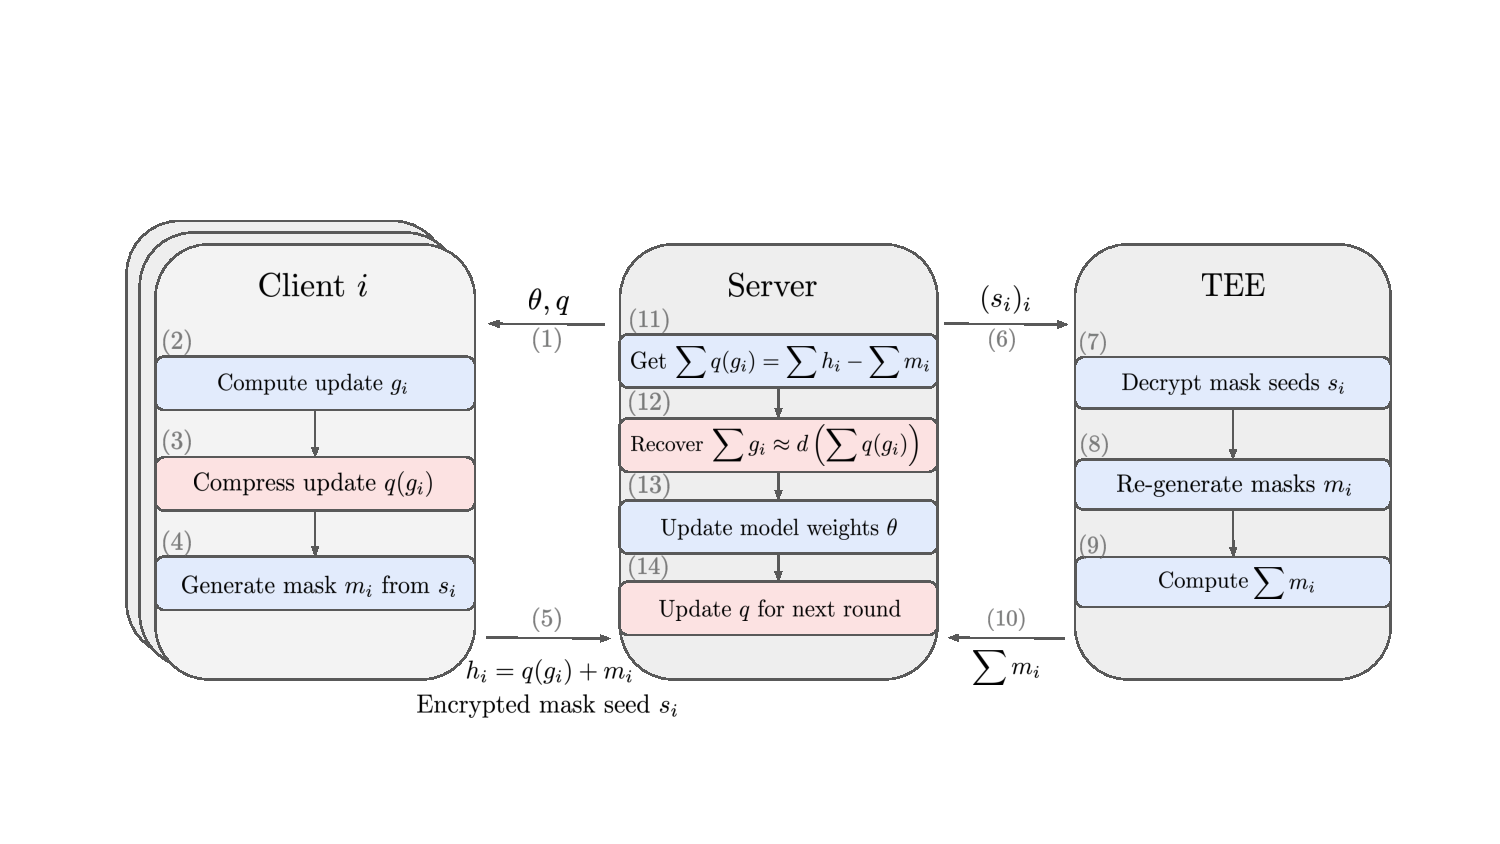
\includegraphics[width=0.9\textwidth]{submissions/GrahamCormode/figs/secagg_summary_new.pdf}
    %\vspace{-5mm}
    \caption{\label{fig:secagg_summary}
    Summary of the proposed approach for one FL round, where we omit the round dependency and \modif{Differential Privacy (DP)} for clarity. Blue boxes denote standard steps and red boxes denote additional steps for uplink compression. Client $i$ computes local model update $g_i$, compresses it with the compression operator $q$, and encrypts it by adding a random mask $m_i$ in the compressed domain, hence reducing the uplink bandwidth (steps 2--4). The server recovers the aggregate in the compressed domain by leveraging any \SecAgg protocol \modif{(steps 7--13, with a TEE-based \SecAgg, see Section~\ref{subsec:secagg})}. Since the decompression operator $d$ is linear, the server can convert the aggregate back to the non-compressed domain, up to compression error (step 12). As with the model weights $\theta$, the compression operator $q$ are also periodically updated and broadcast by the server (step 14).
    In Section~\ref{sec:method}, we apply the proposed method to scalar quantization and pruning without impacting \SecAgg and propose Secure Indexing, a variant of \SecAgg for extreme uplink compression with product quantization. See Section~\ref{subsec:secagg} for details about \SecAgg and Section~\ref{sec:discussion} for a discussion on~DP.
    }
    \vspace{-3mm}
\end{figure*}



% Our focus in this paper is on

%Second, scaling cross-device (synchronous) FL to millions of clients with various capabilities and intermittent availability \cite{Graham-bonavitz2019federated} suffers from diminishing returns: the wall-clock training time plateaus as the number of clients keeps increasing~\cite{Graham-huba2021papaya}. Even though this challenge can be addressed by leveraging the buffered asynchronous aggregation technique proposed by \cite{Graham-nguyen2021federated}, compatible with DP and SecAgg, the asynchronous protocol remains bottlenecked by communication latency between the server and the clients.


%Considering the above privacy and scalability goals, we focus on enabling efficient FL communications while keeping a high privacy bar. In addition to the primary objective of speeding up convergence, reducing communication costs brings other significant benefits. Lowering communication requirements addresses selection bias due to undersampling clients with limited connectivity, improving fairness and inclusivity metrics. Better communication efficiency shrinks the carbon footprint of FL, whose fraction attributable to communication can reach 95\%~\cite{Graham-qiu2021first}. %Finally, training larger model in FL would be a possibility, when the communication cost is reduced, because local memory or compute requirements can be addressed by modifying the local training loop, for instance with gradient checkpointing \cite{Graham-chen2016training}. However, some form of compression would be required to enable efficient communication.


%First, compressing model updates from the client to the server presents several challenges due to compatibility with SecAgg and is an area suitable for further research.
%Second, upload bandwidth is generally more restricted than download. For instance, according to the most recent FCC report, the ratio of download to upload speeds for DSL/cable providers in the US ranges between 3$\times$ to 20$\times$~\cite{Graham-fcc-broadband}. We consider broadband speeds here because devices participate in the FL training while connected to fixed broadband, usually through Wi-Fi~\cite{Graham-huba2021papaya}.




% Hence, FL provides the ability to leverage data from massive client populations while ensuring the security and privacy of the client data.
% Go further: compatibility with DP / compression as a mitigation techniques of attacks
% Model and gradient compression intrinsically different.
%  Why not having the secure enclave perform the aggregation?


\newcommand{\para}[1]{\noindent \textbf{#1}}

\section{Related Work}
\label{sec:related}

Communication is identified as a primary efficiency bottleneck in FL, especially in the cross-device FL setting~\cite{Graham-kairouz2019advances}.
This has led to significant interest in reducing FL's communication requirements. In what follows, we refer to a local model update in distributed training as a \emph{gradient}, including updates from multiple local training steps.

\para{Efficient Distributed Optimization.} There is a large body of literature on reducing the communication cost for distributed training. \cite{Graham-seide2014bit} proposes quantizing gradients to one bit while carrying the quantization error forward across mini-batches with error feedback. Similarly, \cite{Graham-wen2017terngrad} proposes layer-wise ternary gradients and \cite{Graham-bernstein2018signsgd} suggests using only the sign of the gradients. Gradient sparsity is another related area that is extensively studied \cite{Graham-wangni2017gradient,Graham-aji2017sparse,Graham-lin2017deep,Graham-renggli2018sparcml,Graham-parcollet2022zerofl}.
For instance, \cite{Graham-chen2017adacomp} and \cite{Graham-han2020adaptive} explore adapting the degree of sparsity to the distribution of local client data. Another method, QSGD, tunes the quantization level to trade possibly higher variance gradients for reduced communication bandwidth~\cite{Graham-alistarh2016qsgd}. Researchers also studied structured and sketched model updates \cite{Graham-konen2016federated}.
For example, \cite{Graham-wang2018atomo} proposes expressing gradients as a linear combination of basis vectors common to all workers and \cite{Graham-wang2022fedlite} propose to cluster the gradients and to implement error correction on the client side. Besides gradient compression, other methods such as~\cite{Graham-vepakomma2018split,Graham-hu2019dynamic} reduce the communication cost by partitioning the model such that each client learns a portion of it, while \cite{Graham-he2020group} proposes training small models and periodically distilling them to a larger central model. However, as detailed in Section~\ref{sec:background} and below, most of the proposed methods are not readily compatible with \SecAgg and cannot be used in secure FL.

\para{Bi-directional Compression.} In addition to uplink gradient compression, a line of work also focuses on downlink model compression. In a non-distributed setup, \cite{Graham-zhou2016dorefanet, Graham-courbariaux2015binaryconnect} demonstrates that it is possible to meaningfully train with low bit-width models and gradients. In FL, \cite{Graham-jiang2019model} proposes adapting the model size to the device to reduce both communication and computation overhead. Since the local models are perturbed due to compression, researchers propose adapting the optimization algorithm for better convergence \cite{Graham-liu2019double,Graham-sattler2019robust,Graham-tang2019doublesqueeze,Graham-zheng2019communicationefficient,Graham-amiri2020federated,Graham-philippenko2021preserved}.
Finally, pre-conditioning models during FL training can allow for quantized on-device inference, as demonstrated for non-distributed training by \cite{Graham-gupta2015deep, Graham-krishnamoorthi2018quantizing}. As stated in Section~\ref{sec:intro}, we do not focus on downlink model compression since uplink bandwidth is the main communication bottleneck and since \SecAgg only involves uplink communication.

\para{Aggregation in the Compressed Domain.} In the distributed setting, \cite{Graham-yu2018gradiveq} propose to leverage both gradient compression and parallel aggregation by performing the \emph{ring all-reduce} operation in the compressed domain and decompressing the aggregate. To do so, the authors exploit temporal correlations of the gradients to design a linear compression operator.
% Hence, the server receives the individual compressed gradients and is able to recover the sum of the non-compressed gradients:
% \[\sum_i q(g_i) = q\left(\sum g_i\right).\]
Another method, PowerSGD~\cite{Graham-vogels2019powersgd}, leverages a fast low-rank gradient compressor. However, both aforementioned methods are not evaluated in the FL setup and do not mention \SecAgg.
Indeed, the proposed methods focus on decentralized communication between the workers by leveraging the all-reduce operation.
Moreover, PowerSGD uses (stateful) error feedback on all distributed nodes, which is not readily adaptable to cross-device FL when clients generally participate in a few (not necessarily consecutive) rounds.
% not amenable to FL with SecAgg since the all-reduce operations requires communication between all distributed nodes and not solely through a central server.
Finally, \cite{Graham-rothchild2020fetchsgd} proposes FetchSGD, a compression method using sketching, which is compatible with \SecAgg.

% \ilya{Should we say that our methods are also variants of sketching?}
% \ilya{delete?}\st{In this paper, we focus on adapting standard compression methods to SecAgg (namely, scalar quantization and pruning) and propose Secure Indexing, a variant of SecAgg that is provably secure, to obtain extremely small model updates with product quantization.}





\newcommand{\parai}[1]{\noindent\textit{#1}}

\section{Background}
\label{sec:background}

In this section, we recall the \SecAgg protocol first, then the compression methods that we wish to adapt to \SecAgg, namely, scalar quantization, pruning, and product quantization.

\subsection{Secure Aggregation}
\label{subsec:secagg}

\SecAgg refers to a class of protocols that allow the server to aggregate client updates without accessing them individually. While \SecAgg alone does not entirely prevent client data leakage, it is a powerful and widely-used component of current at-scale cross-device FL implementations~\cite{Graham-kairouz2019advances}. Two main approaches exist in practice: software-based protocols relying on Multiparty Computation (MPC)~\cite{Graham-bonavitz2019federated,Graham-bell2020secure,Graham-LightSecAgg}, and those that leverage hardware implementations of Trusted Execution Environments (TEEs)~\cite{Graham-huba2021papaya}.
% While these approaches have substantial differences, they impose similar constraints on compatible update compression techniques: operating over finite fields and assuming that aggregation commutes with decompression.


\SecAgg relies on additive masking, where clients protect their model updates $g_i$ by adding a uniform random mask $m_i$ to it, guaranteeing that each client’s masked update is statistically indistinguishable from any other value.
% Masks are generated so that when all the masked client updates are aggregated by the server (typically through addition), the server obtains the exact aggregate (e.g., the sum of updates).
At aggregation time, the protocol ensures that all the masks are canceled out. For instance, in an MPC-based \SecAgg, the pairwise masks cancel out within the aggregation itself, since for every pair of users $i$ and $j$, after they agree on a matched pair of input perturbations, the masks $m_{i,j}$ and $m_{j,i}$ are constructed so that $m_{i,j}=-m_{j,i}$.
Similarly and as illustrated in Fig.~\ref{fig:secagg_summary}, in a TEE-based \SecAgg, the server receives $h_i = g_i + m_i$ from each client as well as the sum of the masks $\sum_i m_i$ from the TEE and recovers the sum of the updates as
% by unmasking the aggregated updates as
%\begin{equation*}
$
      \sum_i g_i = \sum_i h_i - \sum_i m_i.
$
%\end{equation*}
We defer the discussion of DP noise addition by \SecAgg protocols to Section~\ref{sec:discussion}.

\para{Finite Group.}
\SecAgg requires that the plaintexts---client model updates---be elements of a finite group, while the inputs are real-valued vectors represented with floating-point types.
This requirement is usually addressed by converting client updates to fixed-point integers and operating in a finite domain (modulo~$2^p$) where $p$ is typically set in prior literature to 32 bits. The choice of \SecAgg bit-width~$p$ must balance communication costs with the accuracy loss due to rounding and overflows.

% The other constraint is due to the fact that SecAgg is designed so that the server sees only the aggregate (the sum or the weighted sum) of individual gradients, plus some noise injected by a differentially private mechanism. A drop-in decompression operator $D$ must commute with SecAgg, or be close to being one:
% \[
% D\left(\sum_i g_i+\mathrm{noise}\right) \approx \sum_i D(g_i)+\mathrm{noise}.
% \]
\para{Minimal Complexity.}
\looseness=-1
TEE-based protocols offer greater flexibility in how individual client updates can be processed; however, the code executed inside TEE is part of the trusted computing base (TCB) for all clients. In particular, it means that this code must be stable, auditable, defects- and side-channel-free, which severely limits its complexity. Hence, in practice, we prefer compression techniques that are either oblivious to \SecAgg's implementation or require minimal changes to the TCB.

% In the remainder of the paper, we focus on the TEE-based approach for its simplicity, scalability and compatibility with asynchronous FL. relies on random masking to encrypt the local model updates. The server then incrementally aggregates the encrypted updates and unmasks the aggregate using the sum of the random masks transmitted by the Trusted Secure Aggregator (TSA) that sits within the TEE. More formally, let us denote $??$ a local client update, represented in floating-point precision, generally \texttt{fp32}. First, the client converts $??$ to a fixed point representation. Then, the client generates a random mask $m \in \Z^d$ and computes the sum modulo a number. \ashkan{TODO}

% SecAgg protocols prevent the server from accessing individual client updates by aggregating them and transmitting only the aggregate to the server. While such mechanisms alone do not entirely prevent data leakage, they constitute a vital component of cross-device FL implementations~\cite{Graham-kairouz2019advances}. SecAgg relies either on Secure Multiparty Computation \cite{Graham-bonavitz2019federated,so2021secure} or on a Trusted Executed Environment or TEE~\cite{Graham-huba2021papaya}. In the remainder of the paper, we focus on the TEE-based approach for its simplicity, scalability and compatibility with asynchronous FL.

% TEE-based SecAgg relies on random masking to encrypt the local model updates. The server then incrementally aggregates the encrypted updates and unmasks the aggregate using the sum of the random masks transmitted by the Trusted Secure Aggregator (TSA) that sits within the TEE. More formally, let us denote $??$ a local client update, represented in floating-point precision, generally \texttt{fp32}. First, the client converts $??$ to a fixed point representation. Then, the client generates a random mask $m \in \Z^d$ and computes the sum modulo a number.

% Since the server, by design, never observes

\subsection{Compression Methods}
\label{subsec:comp_methods}
In this subsection, we consider a matrix $W \in \mathbb{R}^{\cin\times \cout}$ representing the weights of a linear layer to discuss three major compression methods with distinct compression/accuracy tradeoffs and identify the challenges \SecAgg faces to be readily amenable to these popular quantization algorithms.

\subsubsection{Scalar Quantization}
\label{subsec:sq}

\looseness=-1 Uniform scalar quantization maps floating-point weight $w$ to $2^b$ evenly spaced bins, where $b$ is the number of bits. Given a floating-point scale $s > 0$ and an integer shift parameter $z$ called the zero-point, we map any floating-point parameter $w$ to its nearest bin indexed by $\{0,\dots, 2^b-1\}$:

\centerline{$w \mapsto \clamp(\round(w /s) + z, [0, 2^b - 1] ).$}

%
The tuple $(s, z)$ is often referred to as the quantization parameters (\texttt{qparams}).
With $b=8$, we recover the popular \texttt{int8} quantization scheme \cite{Graham-jacob2017quantization}, while setting $b = 1$ yields the extreme case of binarization \cite{Graham-courbariaux2015binaryconnect}.
The quantization parameters $s$ and $z$ are usually calibrated after training a model with floating-point weights using the minimum and maximum values of each layer.
% The accuracy drop due to this post-training quantization can be mitigated by pre-conditioning the network during training with techniques such as Quantization-Aware Training or QAT~\cite{Graham-krishnamoorthi2018quantizing}.
% The quantization parameters can also be defined per-channel instead of per-layer to diminish the quantization error at the cost of a small memory overhead.
The compressed representation of weights $W$ consists of the \texttt{qparams} and the integer representation matrix $W_q$ where each entry is stored in~$b$~bits.
Decompressing any integer entry $w_q$ of~$W_q$ back to floating point is performed by applying  the (linear) operator $w_q \mapsto s\times(w_q - z)$.

\para{Challenge.}
The discrete domain of quantized values and the finite group required by \SecAgg are not natively compatible because of the overflows that may occur at aggregation time. For instance, consider the extreme case of binary quantization, where each value is replaced by a bit.
We can represent these bits in \SecAgg with $p=1$, but the aggregation will inevitably result in overflows.

\subsubsection{Pruning}
\label{subsec:rp}

Pruning is a class of methods that remove parts of a model such as connections or neurons according to some pruning criterion, such as weight magnitude~(\cite{Graham-lecun1990optimal,Graham-hassabi1992second}; see \cite{Graham-Blalock20} for a survey). \cite{Graham-konen2016federated} demonstrate client update compression with random sparsity for federated learning. Motivated by previous work and the fact that random masks do not leak information about the data on client devices, we will leverage random pruning of client updates in the remainder of this paper.
% as it is easiest to combine with SecAgg.
% Let $\texttt{rand}$ be a function generating random entries in interval $[0, 1)$.
% For a sparsity level $0\leq\rho\leq 1$, where $\rho=1$ yields a zero matrix, a client prunes entries~$w$ of~$W$ as:
% % \karthik{TODO: decide on notation for rand}
% \[w \mapsto \begin{cases}
% 0 & \text{if } \texttt{rand()} < \rho \\
% w & \text{otherwise}.
% \end{cases}
% \]
% \sayan{should we number the equations ?}
A standard method to store a sparse matrix is the coordinate list (COO) format\footnote{See the  {torch.sparse documentation}, \url{https://pytorch.org/docs/stable/sparse.html}.}, where only the non-zero entries are stored (in floating point or lower precision), along with their integer coordinates in the matrix.
This format is compact, but only for a large enough compression ratio, as we store additional values for each non-zero entry.
Decompression is performed by re-instantiating the uncompressed matrix with both sparse and non-sparse entries.

\para{Challenge.}
\modif{Pruning model updates on the client side is an effective compression approach} as investigated in previous work. However, the underlying assumption is that clients have different masks, either due to their seeds or dependency on client update parameters (\eg weight magnitudes). This is a challenge for \SecAgg as aggregation assumes a dense compressed tensor, which is not possible to construct when the coordinates of non-zero entries are not the same for all clients.

\subsubsection{Product Quantization}
\label{subsec:pq}


Product quantization (PQ) is a compression technique developed for nearest-neighbor search \cite{Graham-jegou2011product} that can be applied for model compression \cite{Graham-stock2019bit}.
Here, we show how we can re-formulate PQ to represent model updates.
We focus on linear layers and refer the reader to~\cite{Graham-stock2019bit} for adaptation to convolutions.
Let the \emph{block size} be $d$ (say, 8), the number of \emph{codewords} be $k$ (say, 256) and assume that the number of input channels, $\cin$, is a multiple of $d$.
To compress $W$ with PQ, we evenly split its columns into subvectors or blocks of size $d \times 1$ and learn a \emph{codebook} via $k$-means to select the $k$ codewords used to represent the $\cin\times\cout/d$ blocks of $W$. PQ with block size $d=1$ amounts to non-uniform scalar quantization with $\log_2 k$ bits per weight.
% More formally, we first reshape $ W$ into a matrix of size $d \times \cin \cout / d$ and with a slight abuse of notation, we will also use  $W$ to denote the reshaped matrix and work only in the reshaped space.
% Note that the reshaping approach applies to convolutional weights as well: e.g., for a 2D convolution with a kernel of size of $k_s$, we need to change the reshaping part to get matrix of size $d \times \cin\cout k_s^2/d$.

The PQ-compressed matrix $W$ is represented with the tuple $(C, A)$, where $C$ is the codebook of size $k \times d$ and $A$ gives the assignments of size $\cin \times\cout / d$.
% \begin{align*}
% C & \text{    the codebook of size } k \times d,  \\
% A & \text{    the assignments of size }\cin \cdot\cout / d.
% \end{align*}
Assignments are integers in $[0, k-1]$ and denote which codebook a subvector was assigned~to.
To decompress the matrix (up to reshaping), we index the codebook with the assignments, written in PyTorch-like notation as
%\begin{equation*}
$
    \widehat {W} = C[A].
$
%\end{equation*}
% (appropriating a PyTorch-like notation) and perform a reshaping operation. PQ is naturally extensible to convolutional layers~\cite{Graham-stock2019bit}.

\para{Challenge.}
There are several obstacles to making PQ compatible with \SecAgg.
First, each client may have a different codebook, and direct access to these codebooks is needed to decode each client's message.
Even if all clients share a (public) codebook, the operation to take assignments to produce an (aggregated) update is not linear, and so cannot be directly wrapped inside \SecAgg.
%In theory PQ is a linear operation, since we can encode each client's choice of codeword for a block with a 1-hot vector of length $k$, and com



\section{Method}
\label{sec:method}

In this section, we propose solutions to
% the challenges identified in Section~\ref{subsec:comp_methods} to
reconcile security (\SecAgg) and communication efficiency.
Our approach is to modify compression techniques to share some hyperparameters globally across all clients so that aggregation can be done by uniformly combining each client's response, while still ensuring that there is scope to achieve accurate compressed representations.
\modif{As detailed below, each of the proposed methods offers the same level of security as standard \SecAgg without compression.}

\subsection{Secure Aggregation and Compression}
\label{subsec:secagg_comp}
We propose to compress the uplink model updates through a compression operator $q$, whose parameters are round-dependent but the same for all clients participating in the same round.
Then, we will add a random mask $m_i$ to each quantized client update $q(g_i)$ in the compressed domain, thus effectively reducing uplink bandwidth while ensuring that $h_i = q(g_i) + m_i$ is statistically indistinguishable from any other representable value in the finite group (see Section~\ref{subsec:secagg}).
In this setting, \SecAgg allows the server to recover the aggregate of the client model updates in the compressed domain: $\sum_i q(g_i)$.
% \begin{equation*}
%     \sum_i q(g_i) = \sum_i h_i- \sum_i m_i
% \end{equation*}
If the decompression operator $d$ is linear, the server is able to recover the aggregate in the non-compressed domain, up to quantization error, as illustrated in Figure~\ref{fig:secagg_summary}:
\begin{equation*}\textstyle
    d\left(\sum_i h_i - \sum_i m_i\right) = d\left(\sum_i q(g_i)\right) =\sum_i d(q(g_i)) \approx \sum_i g_i.
\end{equation*}
% \ashkan{according to the top equation in page 4, $\sum h_i$ minus $\sum m_i$ is exactly $\sum g_i$ and not $\sum q(g_i)$. I understand here we are talking about compression. But a reviewer might complain here that this is not consistent. Should we add $q(.)$ around the first part too?}
The server periodically updates the quantization and decompression operator parameters, either from the aggregated model update, which is deemed public, or by emulating a client update on some similarly distributed public data. Once these parameters are updated, the server broadcasts them to the clients for the next round. \modif{This adds overhead to the downlink communication payload, however, this is negligible compared to the downlink model size to transmit}. For instance, for scalar quantization, $q$ is entirely characterized by one \texttt{fp32} scale and one \texttt{int32} zero-point per layer, the latter of which is unnecessary in the case of a symmetric quantization scheme. Finally, this approach is compatible with both synchronous FL methods such as FedAvg~\cite{Graham-mcmahan2016communicationefficient} and asynchronous methods such as FedBuff~\cite{Graham-nguyen2021federated} as long as \SecAgg maintains the mapping between the successive versions of quantization parameters and the corresponding client updates.

\subsection{Application}
Next, we show how we adapt scalar quantization and random pruning with no changes required to \SecAgg. We illustrate our point with TEE-based \SecAgg while these adapted uplink compression mechanisms are agnostic of the \SecAgg mechanism. Finally, we show how to obtain extreme uplink compression by proposing a variant of \SecAgg, which we call \SecInd. This variant supports product quantization and is provably secure.

\subsubsection{Scalar Quantization and Secure Aggregation}
\label{subsubsec:sq_sa}

As detailed in Section~\ref{subsec:sq}, a model update matrix $g_i$ compressed with scalar quantization is given by an integer representation in the range $[0, 2^{b}-1]$ and by the quantization parameters \emph{scale} ($s$) and \emph{zero-point} ($z$). A sufficient condition for the decompression operator to be linear is to broadcast common quantization parameters per layer for each client. Denote $q(g_i)$ as the integer representation of quantized client model update $g_i$ corresponding to a particular layer for client $1\leq i \leq N$.
%Let us assume that the server's aggregation method is the sum.
Set the scale of the decompression operator to $s$ and its zero-point to $z/N$.
Then, the server is able to decompress as follows (where the decompression operator is defined in Section~\ref{subsec:sq}):
\begin{equation*}\textstyle
    % (s\sum_i  q(g_i)) - \frac{sz}{n} = \sum_i s(q(g_i) - z) \simeq \sum_i g_i.
    d\left(\sum_i q(g_i)\right) = s\sum_i  q(g_i) -  \frac{z}{N}  = \sum_i \left( s(q(g_i)) - z \right) \approx \sum_i g_i
\end{equation*}
Recall that all operations are performed in a finite group. Therefore, to avoid overflows at aggregation time, we quantize with a bit-width $b$ but take \SecAgg bit-width $p > b$, thus creating a margin for potential overflows (see Section~\ref{subsec:ablations}).
%\ilya{Do we really? (Make SecAgg bitwidth larger than b.) Masked updates are defined only modulo $2^b$, adding them in larger group makes little sense.}.
%
This approach is related to the fixed-point aggregation described in \cite{Graham-bonavitz2019federated,Graham-huba2021papaya}, but we calibrate the quantization parameters and perform the calibration per layer and periodically, unlike the related approaches.
% whereas the scale parameter used in fixed-point conversion does not change during the training and is common to the whole network.\ilya{I am confused - does the scale change periodically or it doesn't?}

\modif{\para{Privacy, Security and Bandwidth.}} Scales and zero points are determined from public data on the server. Downlink overhead is negligible: the server broadcasts the per-layer quantization parameters. The upload bandwidth is $p$ bits per weight, where $p$ is the \SecAgg finite group size (Section~\ref{subsec:secagg}). \modif{Since the masks $m_i$ are chosen in the integer range $[0, 2^p-1]$, any masked integer representation taken modulo $2^p$ is statistically indistinguishable from any other vector.}
% The maximum ``price of security'' is thus the overflow buffer of $p-b = \lceil\log_2 N\rceil$ bits per weight.

\subsubsection{Pruning and Secure Aggregation}

To enable linear decompression with random pruning, all clients will share a common pruning mask for each round.
This can be communicated compactly before each round as a seed for a pseudo-random function.
%the server broadcasts one common pruning mask seed before each round.
This pruning mask seed is different from the \SecAgg mask seed introduced in Section~\ref{subsec:secagg} and has a distinct role.
Each client uses the pruning seed to reconstruct a pruning mask, prunes their model update $g_i$, and only needs to encrypt and transmit the unpruned parameters.
The trade-off here is that some parameters are completely unobserved in a given round, as opposed to traditional pruning.
%we obtain no signal about some parameters in a given round, in contrast to traditional pruning.
\SecAgg operates as usual and the server receives the sum of the tensor of unpruned parameters computed by participating clients in the round, which it can expand using the mask seed.
We denote the pruning operator as $\phi$ applied to the original model update $g_i$, and the decompression operator as $d$ applied to a compressed tensor $\phi(g_i)$. Decompression is an expansion operation equivalent to multiplication with a sparse permutation matrix $P_i$ whose entries are dependent on the $i$'th client's mask seed.
Crucially, when all clients share the same mask seed within each round, we have $P_i = P$ for all $i$ and linearity of decompression is maintained:
\begin{equation*} \textstyle
    d \left(\sum_i \phi(g_i) \right) = P \left( \sum_i \phi(g_i) \right) = \sum_i P_i\phi(g_i) = \sum_i d(\phi(g_i)) \approx \sum_i g_i.
\end{equation*}
%
\modif{\para{Privacy, Security and Bandwidth.}} Since the mask is random, no information leaks from the pruning mask. The downlink overhead (the server broadcasts one integer mask seed) is negligible. The upload bandwidth is simply the size of the sparse client model updates. \modif{Finally, there is no loss in security since each client uses standard \SecAgg mechanism on the non-pruned entries.}

\subsubsection{Product Quantization and Secure Indexing}

\begin{algorithm}[t]
\caption{Secure Indexing (\SecInd)}
\label{alg:sec_indexing}
\begin{algorithmic}[1]

% \Procedure{On client}{C}      \Comment{Client-side logic}
%     \State Receive common codebook $C$
%     \State Compute assignment matrix $A^i$  \Comment{$i$ is the client index}
%     \State Encrypt assigment matrix \Comment{For instance with additive masking}
% \EndProcedure

\Procedure{SecureIndexing}{C}      \Comment{This happens inside the TEE}
    \State Receive common codebook $C$ from server \Comment{$C$ is periodically updated by the server}
    \State Initialize histograms $H_{m,n}$ to $0$ \Comment{Each histogram for block $(m, n)$ has size $k$}
    \For{each client $i$}
    \State Receive and decrypt assignment matrix $A^i$ %\Comment{For instance with additive masking}
        \For{each block index $(m, n)$}
            \State $r \leftarrow A^i_{m, n}$ \Comment{Recover assignment of client $i$ for block $(m, m)$}
            \State $H_{m, n}[r] \leftarrow H_{m, n}[r] + 1$ \Comment{Update global count for codeword index $r$}
        \EndFor
    \EndFor
    \State Send back histograms $H_{m, n}$ to the server
\EndProcedure
\end{algorithmic}
\end{algorithm}



% \ashkan{question on notatin: sometimes we have () around A, sometimes we do not, e.g. in the equation below. Sometimes the superscript $i$ is outside () and sometimes inside. Do these have different meaning?}
% We first express product quantization in terms of a linear decompression operator.
%We describe the novel Secure Indexing protocol


We next describe the Secure Indexing (\SecInd) primitive, and discuss how to instantiate it.
Recall that with PQ, each layer has its own codebook $C$ as explained in Section~\ref{sec:method}.
Let us fix one particular layer compressed with codebook $C$, containing $k$ codewords.
We assume that $C$ is common to all clients participating in the round.
Consider the assignment matrix of a given layer $(A^i)_{m,n}$ for client~$i$.
From these, we seek to build the \emph{assignment histograms} $H_{m,n} \in \mathbb R^k$ that satisfy
%\begin{equation*}
$H_{m,n}[r] = \sum_i \mathbf 1\left(A^i_{m,n} = r\right),$
%\end{equation*}
where the indicator function $\mathbf 1$ satisfies $\mathbf 1\left(A^i_{m,n} = r\right) = 1$ if $A^i_{m,n} = r$ and $0$ otherwise.
A \emph{Secure Indexing} primitive will produce~$H_{m,n}$ while ensuring that no other information about client assignments or partial aggregations is revealed.
The server receives assignment histograms from \SecInd and is able to recover the aggregated update for each block indexed by $(m, n)$ as
%\begin{equation*}
$
        \sum_r  H_{m,n}[r] \cdot C[r].
$
%\end{equation*}
%
We describe how \SecInd can be implemented with a TEE in Algorithm~\ref{alg:sec_indexing}.
Each client encrypts the assignment matrix, for instance with additive masking as described in Section~\ref{subsec:secagg}, and sends it to the TEE via the server.
Hence, the server does not have access to the plaintexts client-specific assignments.
TEE decrypts each assignment matrix and for each block indexed by $(m, n)$ produces the assignment histogram.
%\ilya{sentence fragment. I don't know where it is heading.}
% where
% \begin{equation*}
%     \mathbf 1\left(A^i_{m,n} = r\right) =
%     \begin{cases}
%         1 & \text{if } A^i_{m,n} = r  \\
%         0  & \text{otherwise}.
%     \end{cases}
% \end{equation*}
%\ilya{Delete:}\st{Since the enclave decrypts the individual assignment matrices, the proposed method is orthogonal to the encryption process.}
Compared to \SecAgg, where the TEE receives an encrypted seed per client (a few bytes per client) and sends back the sum of the masks $m_i$ (same size as the considered model), \SecInd receives the (masked) assignment matrices and sends back histograms for each round.
%\SecInd implementation feasibility is briefly discussed in Appendix~\ref{appendix:secind}.
\SecInd can be implemented in other models, offering different trust paradigms,
such as the multi-party computation setting (using two or more servers to operate on shares of the input).
Encoding inputs as shares of one-hot vectors would lose the advantages of compression.
Instead, each client can send evaluations of \emph{distributed point functions} to encode each assignment~\cite{Graham-boyle16}.
These are represented compactly, but may require longer codewords to overcome the overheads.

%An advantage of working with multiple servers is that we can compute the final output (\ie the update) without exposing any intermediate representation in terms of the histogram of codewords.
%That is, we could obtain shares of the histogram in the MPC model, and then use these in conjunction with the (public) codebook to build shares of the update, before finally combining these to reveal the update.
%This could also be combined with the introduction of DP noise to ensure privacy as well as security.
% expands it to $(\widetilde A^i)_{m,n,r}$ by replacing each assignment index by a one-hot vector of size $k$:
% \[  \widetilde A^i_{m,n,r} =
%     \begin{cases}
%         1 & \text{if } A^i_{m,n} = r  \\
%         0  & \text{otherwise}.
%     \end{cases}
% \]
% Let us assume further that the codebook $C$ is common to all clients participating in the round.
% % $C$ is computed by the server
% % %on a mock client
% % using public data or from the aggregated (public) model update.
% Then, the server is able to recover the aggregated update for each block indexed by $(m, n)$:
% \[ \ashkan{?=}\sum_r \left(\sum_{i} \widetilde A^i_{m,n,r} \right)\cdot C_r
% \]
% However, in practice we do not wish to instantiate the sparse matrix $(\widetilde A^i)_{m,n,r}$ due to its size.
% Instead, we propose Secure Indexing\karthik{where exactly do we propose this?}, a variant of SecAgg that receives the (non-expanded) assignment matrices $(A)^i_{m,n}$ and sends the aggregate back to the server in a compact form.



\modif{\para{Privacy, Security and Bandwidth.}}
Codebooks are computed from public data while individual assignments are never revealed to the server.
The downlink overhead of sending the codebooks is negligible as demonstrated in Section~\ref{sec:experiments}.
The upload bandwidth in the TEE implementation is the assignment size, represented in $k$ bits (the number of codewords).
For instance, with a block size $d=8$ and $k=32$ codewords, assignment storage costs are 5 bits per 8 weights, which converts to 0.625 bits per weight.
The tradeoff compared to non-secure PQ is the restriction to a global codebook for all clients (instead of one tailored to each client), and the need to instantiate \SecInd instead of \SecAgg. \modif{Since the assignments are encrypted before being sent to the TEE, there is no loss in security. Here, any encryption mechanism (not necessarily relying on additive masking) would work.}


\section{Experiments}
\label{sec:experiments}

\begin{figure*}[t]
    \centering
    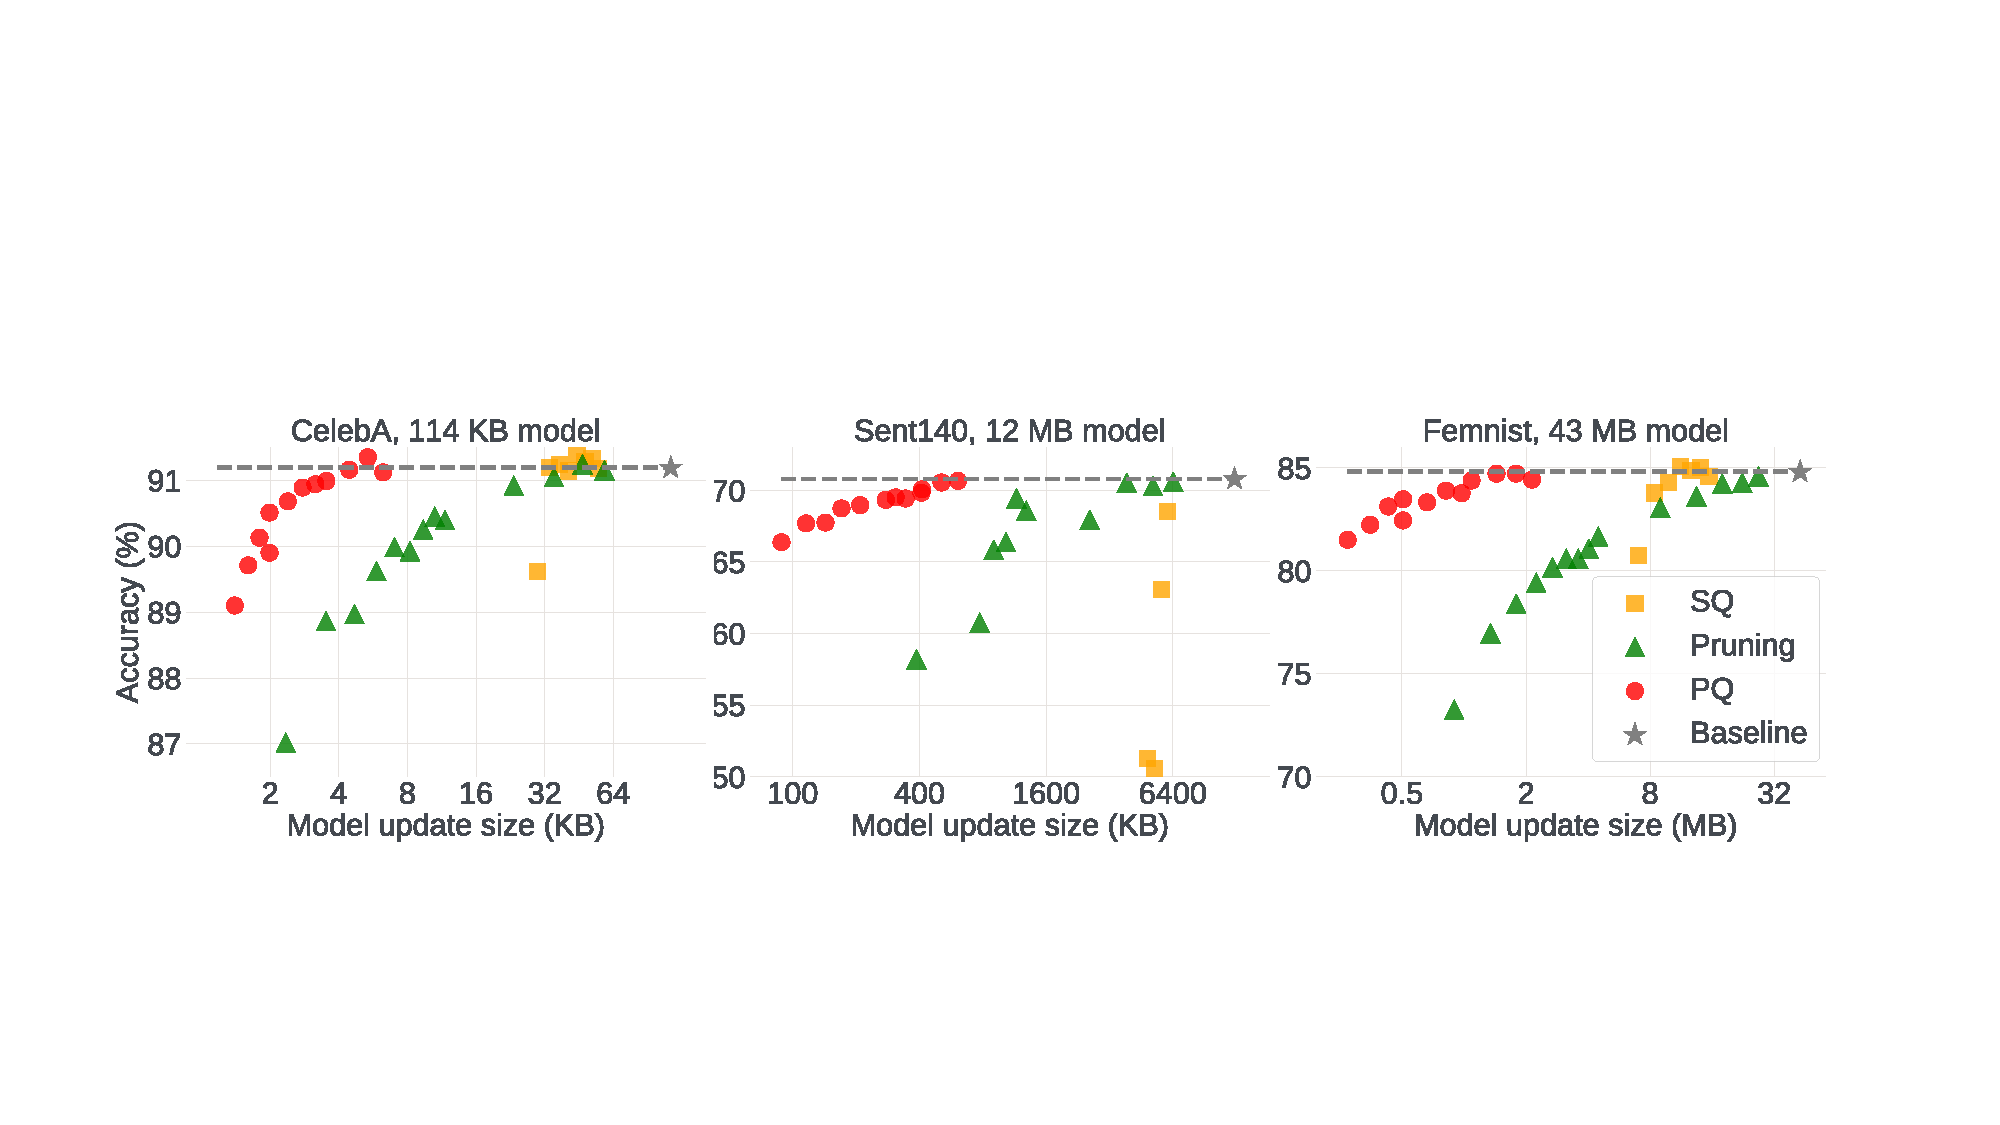
\includegraphics[width=\textwidth]{submissions/GrahamCormode/figs/results_summary.pdf}
    \vspace{-5mm}
    \caption{\label{fig:results_summary}
    We adapt scalar quantization (SQ) and pruning to the \SecAgg protocol to enable efficient and secure uplink communications. We also present results for product quantization (PQ) under the proposed novel \SecInd protocol. \modif{\emph{The $x$ axis is log-scale} and represents the uplink message size}. Baseline refers to \SecAgg FL run without any uplink compression, shown as a horizontal line for easier comparison. Model size is indicated in plot titles. Uncompressed client updates are as large as the models when $p=32$ (see Sec~\ref{subsec:secagg}, shown as stars).
    %We refer to the Appendix~\ref{appendix:table} for the matching tables where we additionally report the standard deviation of each data point.
    }
\end{figure*}

% \pierre{TODO: Table/graph for SQ overflows}
% \pierre{Convergence curves baseline vs compression?}
%In this section, w
We evaluate the performance of the proposed approaches when adapted to \SecAgg protocols.
We study the relationship between uplink compression and model accuracy for the LEAF benchmark tasks.
For scalar and product quantization we also analyze the impact of refresh rate for compression parameters on  model performance.

\subsection{Experimental Setup}
\label{subsec:setup}
We follow the setup of~\cite{Graham-nguyen2021federated} and use the {FLSim library}
% \footnote{Available at \href{https://github.com/facebookresearch/FLSim}{https://github.com/facebookresearch/FLSim}}
for our experiments
% \footnote{Code available at \texttt{github.com/facebookresearch/SecureFLCompression}.}
.
All experiments are run on a single V100 GPU 16 GB (except for Sent140 where we use one V100 32 GB) and typically take a few hours to run.
%More experiment details can be found in Appendix \ref{appendix:exp_details}.

\para{Tasks.} We run experiments on three datasets from the LEAF benchmark~\cite{Graham-caldas2018leaf}: CelebA~\cite{Graham-liu2015faceattributes}, Sent140~\cite{Graham-Go_Bhayani_Huang_2009} and FEMNIST~\cite{Graham-lecun2010mnist}. For CelebA, we train the same convolutional classifier as ~\cite{Graham-nguyen2021federated} with BatchNorm layers replaced by GroupNorm layers and 9,343 clients. For Sent140, we train an LSTM classifier for binary sentiment analysis with $59,400$ clients.
For FEMNIST, we train a GroupNorm version of the ResNet18~\cite{Graham-he2015deep} for digit classification with 3,550 clients.
We do not compress biases and norm layers due to their small overhead.

\para{Baselines.}  We focus here on the (synchronous) FedAvg approach although, as explained in Section~\ref{sec:method}, the proposed compression methods can be readily adapted to asynchronous FL aggregation protocols. \modif{As in prior work, we keep the number of clients per round to at most $100$,
%(see Appendix~\ref{appendix:exp_details}),
a small fraction of the total considered population size~\cite{Graham-chen2019federated,Graham-charles2021largecohort}.}
We report the average and standard deviation of accuracy over three independent runs for all tasks at different uplink byte sizes corresponding to various configurations of the compression operator.
% \sayan{important point : why do we use gradient and client update interchangeably ? they're not the same and for FedAvg it should be client update deltas ?} \karthik {I belieev I have changed gradients to client updates everywhere, except in related works section where we warn we might use graidents to mean updates}

% \subsection{Secure and Efficient Uplink Communications}

\para{Implementation Details.} We refer the reader to \cite{Graham-techreport} for full experiment details.
The downlink overhead of sending the per-layer codebooks for product quantization is negligible.
%as shown in Appendix~\ref{appendix:codebook_size}.
The convergence time in terms of rounds is similar for PQ runs and the non-compressed baseline/
%, as illustrated in Appendix~\ref{appendix:convergence}.
Note that outside a simulated environment, the wall-clock time convergence for PQ runs would be \emph{lower} than the baseline since uplink communication would be more efficient, hence faster.

\subsection{Results and Comparison with Prior Work}

Results for efficient and secure uplink communications are displayed in Figure~\ref{fig:results_summary}.
%Note that each method is either design to be adapted to S\SecAgg
We observe that PQ yields a consistently better trade-off curve between model update size and accuracy. For instance, on CelebA, PQ achieves $\times 30$ compression with respect to the non-compressed baseline at iso-accuracy. The iso-accuracy compression rate is $\times 32$ on Sent140 and $\times 40$ on FEMNIST (see~\cite{Graham-techreport} for detailed tables).
Scalar quantization accuracy degrades significantly for larger compression rates due to the overflows at aggregation.
%as detailed in Appendix~\ref{appendix:overflow}.
Pruning gives intermediate tradeoffs between scalar quantization and product quantization.

The line of work that develops FL compression techniques is exemplified by FetchSGD~\cite{Graham-rothchild2020fetchsgd} as detailed in Section~\ref{sec:related}, where the authors do not address \SecAgg.
Their results are not directly comparable to ours due to incomparable experimental setups (e.g., datasets and architectures).
However, Figure 6~\cite{Graham-techreport} mentions upload compression rates at iso-accuracy that are weaker than those obtained here with product quantization.

\subsection{Ablation Studies}
\label{subsec:ablations}

\begin{figure*}[t]
    \label{mask-refresh}
    \centering
    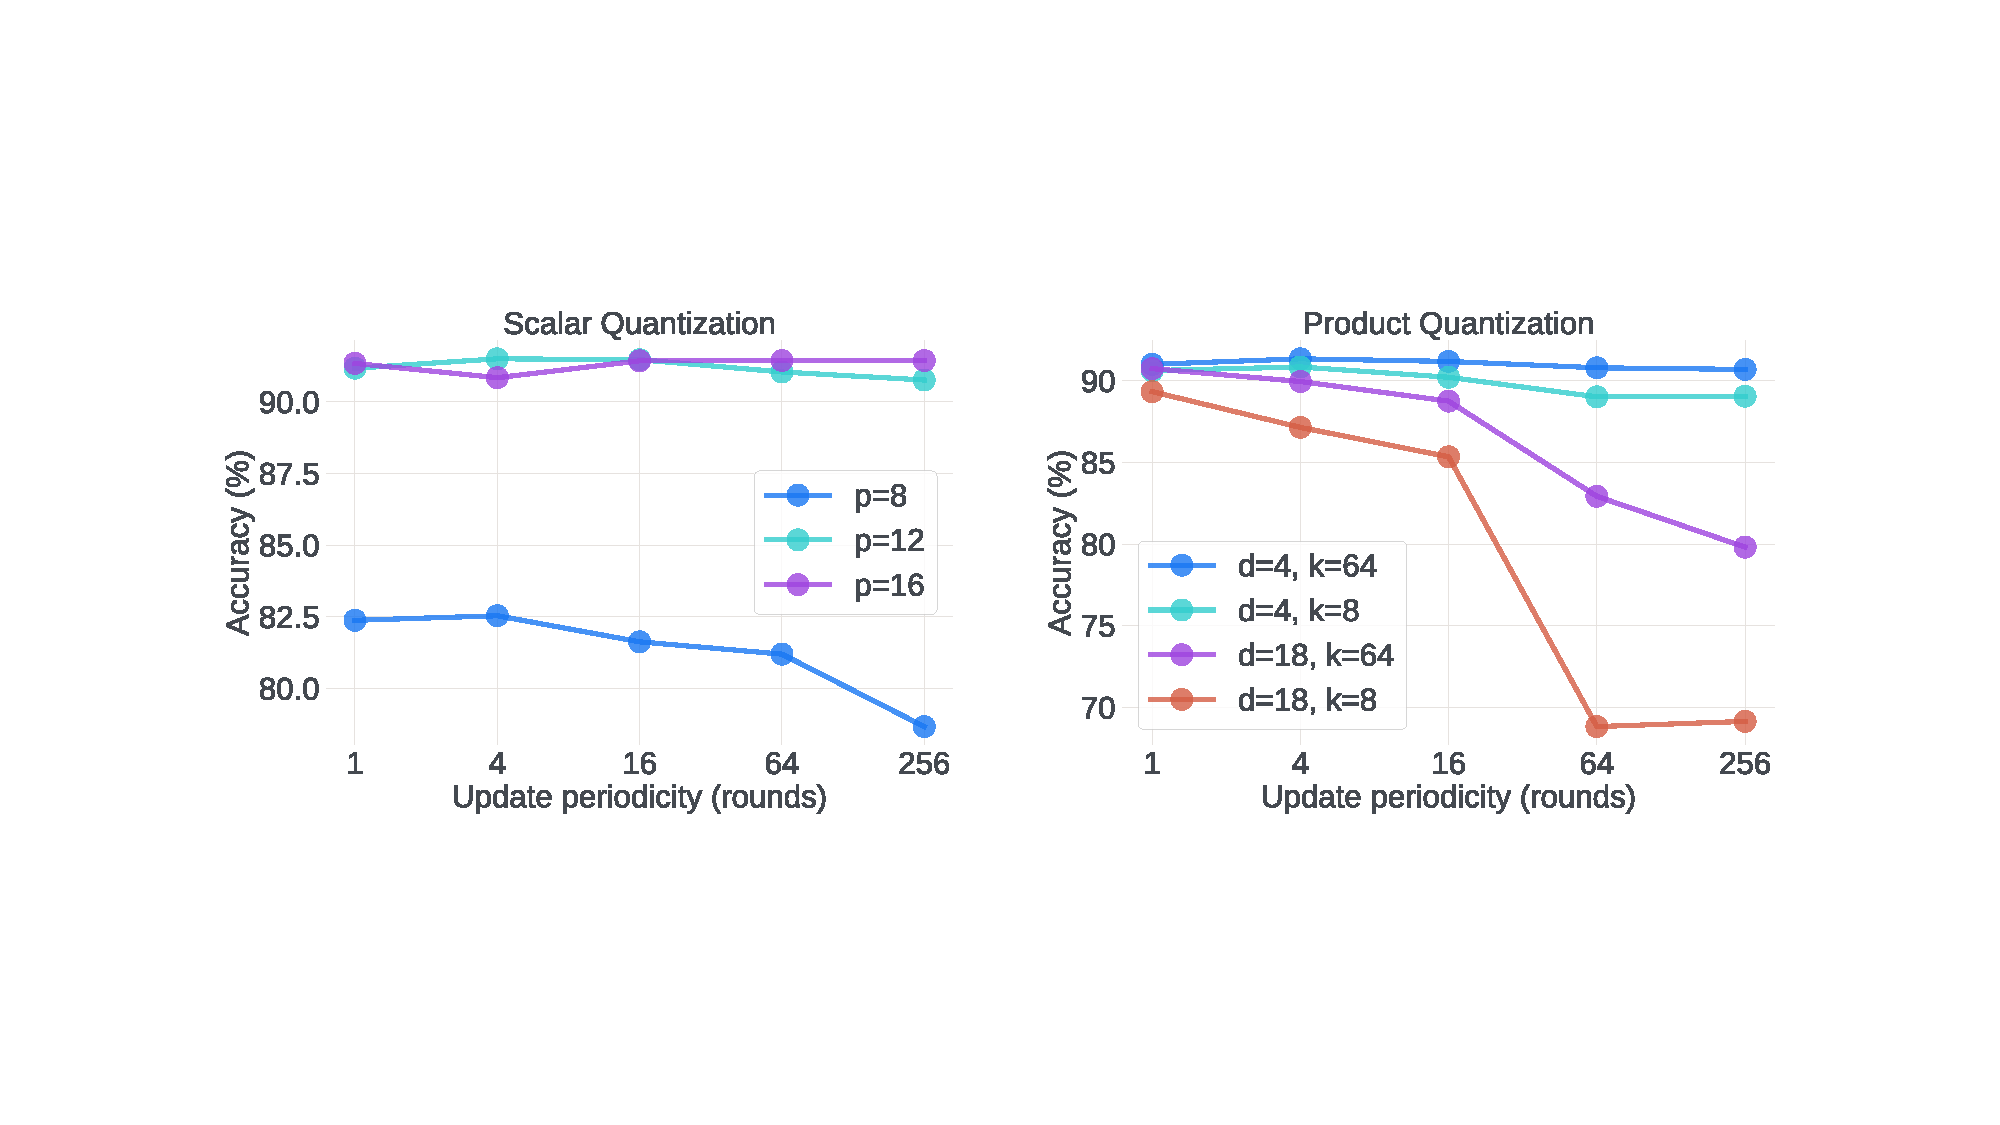
\includegraphics[width=0.9\textwidth]{submissions/GrahamCormode/figs/refresh.pdf}
    \caption{\label{fig:refresh}
    Impact of the refresh rate of the compression operator by the server on the CelebA dataset. \textbf{Left}:  scalar quantization (quantization parameters), fixing the quantization bit-width $b=8$ ($p$ denotes the \SecAgg bit-width). \textbf{Right}: for product quantization (codebooks), where $k$ denotes the number of codewords and $d$ the block size.}
    \vspace{-3mm}
\end{figure*}


We investigate the influence of the frequency of updates of the compression operator $q$ for scalar quantization and pruning, and study the influence of the \SecAgg bit-width $p$ on the number of overflows for scalar quantization.

\para{Update frequency of the compression operators.} In Figure~\ref{fig:refresh}, we show that for scalar quantization, the update periodicity only plays a role with low \SecAgg bit-width values $p$ compared to the quantization bit-width $b$. For product quantization, the update periodicity plays an important role for aggressive compression setups corresponding to large block sizes $d$ or to a smaller number of codewords $k$. For pruning, we measure the impact of masks that are refreshed periodically.
We observed that if we refresh the compression operator more frequently, staleness is reduced, leading to accuracy improvements.
%We present our findings in Appendix~\ref{sparse_refresh}.

\para{Overflows for scalar quantization.}
As discussed in Section~\ref{subsubsec:sq_sa}, we choose the \SecAgg bit-width~$p$ to be greater than quantization bit-width~$b$ in order to avoid aggregation overflows. While it suffices to set $p$ to be $\lceil\log_2 n_c\rceil$ more than $b$, where $n_c$ is the number of clients participating in the round, reducing $p$ is desirable to reduce uplink size.
We studied the impact of  $p$ on the percentage of parameters that suffer overflows, and
observed that there is a benefit to having some non-zero overflow margin size, but no clear correlation between margin size and accuracy.
%present our findings in Appendix~\ref{appendix:overflow}.

% \para{Update frequency of pruning operator $\varrho$.}

% \begin{table*}[t]
%     \small
%     \centering
%     % \vspace{3pt}
%     \begin{tabular}{l@{\hspace{20pt}} c ccc cl@{\hspace{20pt}} ccc}
%     \toprule
%  \bf Compression Method &~~& \multicolumn{3}{c}{\bf CelebA} &~~& \multicolumn{3}{c}{\bf Sent140}\\
%  && \multicolumn{3}{c}{\small ResNet18} &~~& \multicolumn{3}{c}{\small LSTM}\\
% %  && \multicolumn{3}{c}{\small Wikitext-103} &~~& \multicolumn{3}{c}{\small ImageNet-1k}\\
% \cmidrule{3-5}
% \cmidrule{7-9}
% && Gradient size & Compression & Top-1 && Gradient Size & Compression & PPL \\
%     \midrule
%     Baseline & &  $-$ & $\times\ \ 1$ & $-$ & &  $-$ & $\times\ \ 1$ & $-$   \\
%     % \midrule
%     % Binarization & & \\
%     % + \method & & \\
%     \midrule
%     SQ (8 bits) & &  $-$ & $\times\ \ -$ & $-$ & &  $-$ & $\times\ \ -$ & $-$   \\
%     SQ (4 bits) & &  $-$ & $\times\ \ -$ & $-$ & &  $-$ & $\times\ \ -$ & $-$   \\
%     \midrule
%     Pruning ($s=90\%$) & &  $-$ & $\times\ \ -$ & $-$ & &  $-$ & $\times\ \ -$ & $-$   \\
%     Pruning ($s=50\%$) & &  $-$ & $\times\ \ -$ & $-$ & &  $-$ & $\times\ \ -$ & $-$   \\
%     Pruning ($s=10\%$) & &  $-$ & $\times\ \ -$ & $-$ & &  $-$ & $\times\ \ -$ & $-$   \\
%     \midrule
%     PQ ($k=256$, $d=4$) & &  $-$ & $\times\ \ -$ & $-$ & &  $-$ & $\times\ \ -$ & $-$   \\
%     PQ ($k=256$, $d=8$) & &  $-$ & $\times\ \ -$ & $-$ & & $-$ &  $\times\ \ -$ &  $-$  \\
%     \bottomrule
%     \end{tabular}
%  \caption{\small \textbf{Comparison of different quantization schemes with Secure Aggregation}. Blabla.}
%     \label{tab:quantization_comparison}
% \end{table*}


% \subsection{Combination of Compression Techniques}

% \pierre{Song Han Deep Compression for combination}

% \subsubsection{Sparsity \& Scalar Quantization}
% Say/demonstrate that its better to perform pruning first and then SQ than the opposite.

% \subsubsection{Sparsity \& Product Quantization}
% Block sparsity and PQ.

% \subsection{FL Finetuning}

% Maybe also talk about the realistic scenario of FL finetuning (in practice, start from pretrained model on public data to bootstrap learning, in which case gradients may be smaller/sparser hence easier to compress?).
% Partial finetuning.

% \subsection{Heterogeneous Hardware}

% Experiment describing various bit-widths/sparsity level/codebook size per client depending on available bandwidth.

% \pierre{delta with respect to baseline}
% \pierre{discussion about privacy of shared parameters}
% \pierre{DP noise in the enclave until the very end. Privacy vs security = secure FL focus}
% \pierre{Secure Coding}


\section{Concluding Remarks}
\label{sec:discussion}
In this paper, we reconcile efficiency and security for uplink communication in Federated Learning.
We propose to adapt existing compression mechanisms such as scalar quantization and pruning to the secure aggregation protocol by imposing a linearity constraint on the decompression operator.
Our experiments demonstrate that we can adapt both quantization and pruning mechanisms to obtain a high degree of uplink compression with minimal degradation in performance and higher security guarantees. For achieving the highest rates of compression, we introduce \SecInd, a variant of \SecAgg well-suited for TEE-based implementation that supports product quantization while maintaining a high security bar.
%We plan to extend our work to other federated learning scenarios, such as asynchronous FL, and further investigate the interaction of compression and privacy.
%\section{Extensions}
As mentioned in Section~\ref{sec:intro}, we {may want } both \SecAgg and Differential Privacy~\cite{Graham-abadi2016deep} to realize the full promise of FL as a privacy-enhancing technology.
While our primary focus is on enabling efficient and secure uplink communication, we emphasize that the proposed approaches are compatible with user-level DP.
For instance, {at the cost of increasing the complexity of the trusted computing base}, DP noise can be added natively by the TEE with our modified random pruning or scalar quantization approaches.
For PQ  and \SecInd, {we can have the TEE to add noise in the assignment space (\ie outputting a noisy histogram), or to map the histogram to the codeword space and add noise there.
Each option offers a different tradeoff between privacy, trust, and accuracy; we leave detailed evaluation to future work.}




%\modif{\textbf{Compatibility with DP.}
%\sout{it would require, however, to transfer the aggregation to TEE or to design a DP mechanism in the assignment space, since DP noise must be added by the TEE and not by the server.}}

%\modif{\textbf{Efficiency and Privacy.}} A separate line of work {aims} to combine communication efficiency and privacy.
%For instance, \cite{Graham-triastcyn2021dprec} develop a method that unifies compressed communication and DP (where integration with \SecAgg is left as an open problem), while \cite{Graham-chaudhuri2022privacyaware} design a privacy-aware scalar compression mechanism within the \emph{local} differential privacy model.

%\graham{\sout{
%\modif{\textbf{Broader Social Impact. }} In this work, we propose to enhance the privacy of individuals who may contribute to training ML models and simultaneously enable more individuals to participate in private training, who might otherwise have been excluded due to resource constraints. }}
% Indeed, Federated Learning could enable a malicious server to access individual model updates that can leak personal information. Hence, we propose a secure way to communicate the individual model updates.

% - Generic and less data-dependent codebook
% - Model compression
% - Compression and DP
% - Error correction

% There are multiple extensions of PQ, such as having multiple codebooks per matrix  (which increases the cost of storing the codebooks) or performing the assignments with other norms than the $L_2$ norm.



% As a side note, \cite{Graham-jia2022federated} propose to perform domain adaptation by fine-tuning a small fraction of the model parameters, which is naturally compatible with Secure Aggregation, but requires to start from a pretrained model.




% and global and local differential privacy,
% and investigate strategies to select optimal compression parameters
% (quantization scales, centroids and pruning masks)
% for better performance in these scenarios.

% % This
% % - Generic and less data-dependent codebook
% % - Model compression
% % - Compression and DP
% % - Error correction

% % \section*{Acknowledgements}

%\bibliography{bibliography}\bibliographystyle{abbrv}\end{document}

\begin{thebibliography}{10}
\setlength{\itemsep}{1pt}
\begin{small}
\bibitem{Graham-abadi2016deep}
M.~Abadi, A.~Chu, I.~Goodfellow, H.~B. McMahan, I.~Mironov, K.~Talwar, and
  L.~Zhang.
\newblock Deep learning with differential privacy.
\newblock In {\em ACM CCS}, 2016.

\bibitem{Graham-aji2017sparse}
A.~F. Aji and K.~Heafield.
\newblock Sparse communication for distributed gradient descent.
\newblock In {\em EMNLP}, 2017.

\bibitem{Graham-alistarh2016qsgd}
D.~Alistarh, D.~Grubic, J.~Li, R.~Tomioka, and M.~Vojnovic.
\newblock {QSGD}: {C}ommunication-efficient {SGD} via gradient quantization and
  encoding.
\newblock In {\em NeurIPS}, 2017.

\bibitem{Graham-amiri2020federated}
M.~M. Amiri, D.~Gunduz, S.~R. Kulkarni, and H.~V. Poor.
\newblock Federated learning with quantized global model updates.
\newblock {\em CoRR}, 2006.10672, 2020.

\bibitem{Graham-bell2020secure}
J.~H. Bell, K.~A. Bonawitz, A.~Gasc{\'o}n, T.~Lepoint, and M.~Raykova.
\newblock Secure single-server aggregation with (poly) logarithmic overhead.
\newblock In {\em ACM CCS}, 2020.

\bibitem{Graham-bernstein2018signsgd}
J.~Bernstein, Y.-X. Wang, K.~Azizzadenesheli, and A.~Anandkumar.
\newblock sign{SGD}: {C}ompressed optimisation for non-convex problems.
\newblock In {\em ICML}, PMLR, 2018.

\bibitem{Graham-Blalock20}
D.~Blalock, J.~J. Gonzalez~Ortiz, J.~Frankle, and J.~Guttag.
\newblock What is the state of neural network pruning?
\newblock In {\em MLSys}, 2020.

\bibitem{Graham-bonavitz2019federated}
K.~A. Bonawitz, F.~Salehi, J.~Kone{\v{c}}n{\'y}, B.~McMahan, and M.~Gruteser.
\newblock Federated learning with autotuned communication-efficient secure
  aggregation.
\newblock In {\em ACSCC}. {IEEE}, 2019.

\bibitem{Graham-boyle16}
E.~Boyle, N.~Gilboa, and Y.~Ishai.
\newblock Function secret sharing: Improvements and extensions.
\newblock In {\em ACM CCS}, 2016.

\bibitem{Graham-caldas2018leaf}
S.~Caldas, P.~Wu, T.~Li, J.~Kone{\v{c}}n{\'y}, H.~B. McMahan, V.~Smith, and
  A.~Talwalkar.
\newblock {LEAF:} {A} benchmark for federated settings.
\newblock {\em CoRR}, abs/1812.01097, 2018.

\bibitem{Graham-carlini2021membership}
N.~Carlini, S.~Chien, M.~Nasr, S.~Song, A.~Terzis, and F.~Tram{\`{e}}r.
\newblock Membership inference attacks from first principles.
\newblock {\em CoRR}, abs/2112.03570, 2021.

\bibitem{Graham-carlini2020extracting}
N.~Carlini, F.~Tram{\`{e}}r, E.~Wallace, M.~Jagielski, A.~Herbert{-}Voss,
  K.~Lee, A.~Roberts, T.~B. Brown, D.~Song, {\'{U}}.~Erlingsson, A.~Oprea, and
  C.~Raffel.
\newblock Extracting training data from large language models.
\newblock In {\em {USENIX} Security Symposium}, 2021.

\bibitem{Graham-charles2021largecohort}
Z.~Charles, Z.~Garrett, Z.~Huo, S.~Shmulyian, and V.~Smith.
\newblock On large-cohort training for federated learning.
\newblock {\em CoRR}, 2106.07820, 2021.

\bibitem{Graham-chen2017adacomp}
C.~Chen, J.~Choi, D.~Brand, A.~Agrawal, W.~Zhang, and K.~Gopalakrishnan.
\newblock {AdaComp}: Adaptive residual gradient compression for data-parallel
  distributed training.
\newblock In {\em AAAI}, 2018.

\bibitem{Graham-chen2019federated}
M.~Chen, R.~Mathews, T.~Ouyang, and F.~Beaufays.
\newblock Federated learning of out-of-vocabulary words.
\newblock {\em CoRR}, 1903.10635, 2019.

\bibitem{Graham-courbariaux2015binaryconnect}
M.~Courbariaux, Y.~Bengio, and J.-P. David.
\newblock {BinaryConnect}: Training deep neural networks with binary weights
  during propagations.
\newblock {\em CoRR}, 1511.00363, 2015.

\bibitem{Graham-dwork2006calibrating}
C.~Dwork, F.~McSherry, K.~Nissim, and A.~Smith.
\newblock Calibrating noise to sensitivity in private data analysis.
\newblock In {\em Proceedings of the Third Conference on Theory of
  Cryptography}, 2006.

\bibitem{Graham-fcc-broadband}
FCC.
\newblock The eleventh {Measuring Broadband America} fixed broadband report,
  2021.

\bibitem{Graham-geiping2020inverting}
J.~Geiping, H.~Bauermeister, H.~Dr\"{o}ge, and M.~Moeller.
\newblock Inverting gradients---{H}ow easy is it to break privacy in federated
  learning?
\newblock In {\em NeurIPS}, 2020.

\bibitem{Graham-Go_Bhayani_Huang_2009}
A.~Go, R.~Bhayani, and L.~Huang.
\newblock Twitter sentiment classification using distant supervision.
\newblock CS224N Project Report, Stanford, 2009.

\bibitem{Graham-gupta2015deep}
S.~Gupta, A.~Agrawal, K.~Gopalakrishnan, and P.~Narayanan.
\newblock Deep learning with limited numerical precision.
\newblock In {\em ICML}, 2015.

\bibitem{Graham-han2020adaptive}
P.~Han, S.~Wang, and K.~K. Leung.
\newblock Adaptive gradient sparsification for efficient federated learning: An
  online learning approach.
\newblock In {\em ICDCS}, 2020.

\bibitem{Graham-hassabi1992second}
B.~Hassibi and D.~G. Stork.
\newblock Second order derivatives for network pruning: {O}ptimal {B}rain
  {S}urgeon.
\newblock In {\em NeurIPS}, 1992.

\bibitem{Graham-he2020group}
C.~He, M.~Annavaram, and S.~Avestimehr.
\newblock Group knowledge transfer: Federated learning of large {CNN}s at the
  edge.
\newblock In {\em NeurIPS}, 2020.

\bibitem{Graham-he2015deep}
K.~He, X.~Zhang, S.~Ren, and J.~Sun.
\newblock Deep residual learning for image recognition.
\newblock In {\em {IEEE} CVPR}, 2016.

\bibitem{Graham-hu2019dynamic}
C.~Hu, W.~Bao, D.~Wang, and F.~Liu.
\newblock Dynamic adaptive {DNN} surgery for inference acceleration on the
  edge.
\newblock {\em IEEE INFOCOM}, 2019.

\bibitem{Graham-huba2021papaya}
D.~Huba, J.~Nguyen, K.~Malik, R.~Zhu, M.~Rabbat, A.~Yousefpour, C.-J. Wu,
  H.~Zhan, P.~Ustinov, H.~Srinivas, K.~Wang, A.~Shoumikhin, J.~Min, and
  M.~Malek.
\newblock Papaya: Practical, private, and scalable federated learning.
\newblock In {\em MLSys}, 2022.

\bibitem{Graham-jacob2017quantization}
B.~Jacob, S.~Kligys, B.~Chen, M.~Zhu, M.~Tang, A.~Howard, H.~Adam, and
  D.~Kalenichenko.
\newblock Quantization and training of neural networks for efficient
  integer-arithmetic-only inference.
\newblock In {\em IEEE CVPR}, June 2018.

\bibitem{Graham-jegou2011product}
H.~J{\'{e}}gou, M.~Douze, and C.~Schmid.
\newblock Product quantization for nearest neighbor search.
\newblock {\em {IEEE} Trans. Pattern Anal. Mach. Intell.}, 33(1):117--128,
  2011.

\bibitem{Graham-jiang2019model}
Y.~Jiang, S.~Wang, B.~J. Ko, W.~Lee, and L.~Tassiulas.
\newblock Model pruning enables efficient federated learning on edge devices.
\newblock {\em CoRR}, abs/1909.12326, 2019.

\bibitem{Graham-kairouz2019advances}
P.~{Kairouz et al.}
\newblock Advances and open problems in federated learning.
\newblock {\em Found. Trends Mach. Learn.}, 14(1–2), 2021.

\bibitem{Graham-konen2016federated}
J.~Konečný, H.~B. McMahan, F.~X. Yu, P.~Richtarik, A.~T. Suresh, and
  D.~Bacon.
\newblock Federated learning: Strategies for improving communication
  efficiency.
\newblock In {\em NIPS Workshop on Private Multi-Party Machine Learning}, 2016.

\bibitem{Graham-krishnamoorthi2018quantizing}
R.~Krishnamoorthi.
\newblock Quantizing deep convolutional networks for efficient inference.
\newblock {\em CoRR}, 1806.08342, 2018.

\bibitem{Graham-lecun1990optimal}
Y.~Le~Cun, J.~S. Denker, and S.~A. Solla.
\newblock Optimal brain damage.
\newblock In {\em NeurIPS}, 1989.

\bibitem{Graham-lecun2010mnist}
Y.~LeCun and C.~Cortes.
\newblock {MNIST} handwritten digit database.
\newblock http://yann.lecun.com/exdb/mnist/, 2010.

\bibitem{Graham-lin2017deep}
Y.~Lin, S.~Han, H.~Mao, Y.~Wang, and W.~Dally.
\newblock Deep gradient compression: Reducing the communication bandwidth for
  distributed training.
\newblock In {\em ICLR}, 2018.

\bibitem{Graham-liu2019double}
X.~Liu, Y.~Li, J.~Tang, and M.~Yan.
\newblock A double residual compression algorithm for efficient distributed
  learning.
\newblock In {\em AISTATS}, 2020.

\bibitem{Graham-liu2015faceattributes}
Z.~Liu, P.~Luo, X.~Wang, and X.~Tang.
\newblock Deep learning face attributes in the wild.
\newblock In {\em {IEEE} ICCV}, 2015.

\bibitem{Graham-mcmahan2016communicationefficient}
B.~McMahan, E.~Moore, D.~Ramage, S.~Hampson, and B.~A. y~Arcas.
\newblock Communication-efficient learning of deep networks from decentralized
  data.
\newblock In {\em AISTATS}, 2017.

\bibitem{Graham-MelisSCS19}
L.~Melis, C.~Song, E.~D. Cristofaro, and V.~Shmatikov.
\newblock Exploiting unintended feature leakage in collaborative learning.
\newblock In {\em {IEEE} S\&P}, 2019.

\bibitem{Graham-nguyen2021federated}
J.~Nguyen, K.~Malik, H.~Zhan, A.~Yousefpour, M.~Rabbat, M.~Malek, and D.~Huba.
\newblock Federated learning with buffered asynchronous aggregation.
\newblock In {\em AISTATS}, 2022.

\bibitem{Graham-parcollet2022zerofl}
T.~Parcollet, J.~Fernandez-Marques, P.~PB~Gusmao, Y.~Gao, and N.~D. Lane.
\newblock {ZeroFL}: Efficient on-device training for federated learning with
  local sparsity.
\newblock In {\em ICLR}, 2022.

\bibitem{Graham-philippenko2021preserved}
C.~Philippenko and A.~Dieuleveut.
\newblock Preserved central model for faster bidirectional compression in
  distributed settings.
\newblock In {\em NeurIPS}, 2021.

\bibitem{Graham-techreport}
K.~Prasad, S.~Ghosh, G.~Cormode, I.~Mironov, A.~Yousefpour, and P.~Stock.
\newblock Reconciling security and communication efficiency in federated
  learning.
\newblock {\em CoRR}, 2207.12779, 2022.

\bibitem{Graham-qiu2021first}
X.~Qiu, T.~Parcollet, J.~Fernandez-Marques, P.~P.~B. de~Gusmao, D.~J. Beutel,
  T.~Topal, A.~Mathur, and N.~D. Lane.
\newblock A first look into the carbon footprint of federated learning.
\newblock {\em arXiv}, 2102.07627, 2021.

\bibitem{Graham-renggli2018sparcml}
C.~Renggli, S.~Ashkboos, M.~Aghagolzadeh, D.~Alistarh, and T.~Hoefler.
\newblock {SparCML}: High-performance sparse communication for machine
  learning.
\newblock In {\em SC}, 2019.

\bibitem{Graham-rothchild2020fetchsgd}
D.~Rothchild, A.~Panda, E.~Ullah, N.~Ivkin, I.~Stoica, V.~Braverman,
  J.~Gonzalez, and R.~Arora.
\newblock {F}etch{SGD}: Communication-efficient federated learning with
  sketching.
\newblock In {\em ICML}, 2020.

\bibitem{Graham-sattler2019robust}
F.~Sattler, S.~Wiedemann, K.-R. M{\"u}ller, and W.~Samek.
\newblock Robust and communication-efficient federated learning from
  non-{i.i.d.} data.
\newblock {\em IEEE Transactions on Neural Networks and Learning Systems},
  31:3400--3413, 2020.

\bibitem{Graham-seide2014bit}
F.~Seide, H.~Fu, J.~Droppo, G.~Li, and D.~Yu.
\newblock 1-bit stochastic gradient descent and its application to
  data-parallel distributed training of speech {DNNs}.
\newblock In {\em {INTERSPEECH}}, 2014.

\bibitem{Graham-stock2019bit}
P.~Stock, A.~Joulin, R.~Gribonval, B.~Graham, and H.~Jégou.
\newblock And the bit goes down: Revisiting the quantization of neural
  networks.
\newblock In {\em ICLR}, 2020.

\bibitem{Graham-tang2019doublesqueeze}
H.~Tang, C.~Yu, X.~Lian, T.~Zhang, and J.~Liu.
\newblock \textsc{DoubleSqueeze}: Parallel stochastic gradient descent with
  double-pass error-compensated compression.
\newblock In {\em ICML}, 2019.

\bibitem{Graham-vepakomma2018split}
P.~Vepakomma, O.~Gupta, T.~Swedish, and R.~Raskar.
\newblock Split learning for health: Distributed deep learning without sharing
  raw patient data, 2018.

\bibitem{Graham-vogels2019powersgd}
T.~Vogels, S.~P. Karimireddy, and M.~Jaggi.
\newblock {PowerSGD}: Practical low-rank gradient compression for distributed
  optimization.
\newblock In {\em NeurIPS}, 2019.

\bibitem{Graham-wang2018atomo}
H.~Wang, S.~Sievert, S.~Liu, Z.~Charles, D.~Papailiopoulos, and S.~Wright.
\newblock {ATOMO}: Communication-efficient learning via atomic sparsification.
\newblock In {\em NeurIPS}, 2018.

\bibitem{Graham-wang2022fedlite}
J.~Wang, H.~Qi, A.~S. Rawat, S.~Reddi, S.~Waghmare, F.~X. Yu, and G.~Joshi.
\newblock Fedlite: A scalable approach for federated learning on
  resource-constrained clients.
\newblock {\em CoRR}, 2201.11865, 2022.

\bibitem{Graham-wangni2017gradient}
J.~Wangni, J.~Wang, J.~Liu, and T.~Zhang.
\newblock Gradient sparsification for communication-efficient distributed
  optimization.
\newblock In {\em NeurIPS}, 2018.

\bibitem{Graham-wen2017terngrad}
W.~Wen, C.~Xu, F.~Yan, C.~Wu, Y.~Wang, Y.~Chen, and H.~Li.
\newblock {TernGrad}: Ternary gradients to reduce communication in distributed
  deep learning.
\newblock In {\em NeurIPS}, 2017.

\bibitem{Graham-LightSecAgg}
C.~Yang, J.~So, C.~He, S.~Li, Q.~Yu, and S.~Avestimehr.
\newblock {LightSecAgg}: Rethinking secure aggregation in federated learning.
\newblock In {\em MLSys}, 2022.

\bibitem{Graham-yu2018gradiveq}
M.~Yu, Z.~Lin, K.~Narra, S.~Li, Y.~Li, N.~S. Kim, A.~Schwing, M.~Annavaram, and
  S.~Avestimehr.
\newblock {GradiVeQ}: Vector quantization for bandwidth-efficient gradient
  aggregation in distributed {CNN} training.
\newblock In {\em NeurIPS}, 2018.

\bibitem{Graham-zheng2019communicationefficient}
S.~Zheng, Z.~Huang, and J.~T. Kwok.
\newblock Communication-efficient distributed blockwise momentum {SGD} with
  error-feedback.
\newblock In {\em NeurIPS}, 2019.

\bibitem{Graham-zhou2016dorefanet}
S.~Zhou, Z.~Ni, X.~Zhou, H.~Wen, Y.~Wu, and Y.~Zou.
\newblock {DoReFa-Net}: Training low bitwidth convolutional neural networks
  with low bitwidth gradients.
\newblock {\em CoRR}, abs/1606.06160, 2016.
\end{small}
\end{thebibliography}
% \pagebreak
%\graham{\sout{Checklist}}
%\section*{Checklist}

% %%% BEGIN INSTRUCTIONS %%%
% The checklist follows the references.  Please
% read the checklist guidelines carefully for information on how to answer these
% questions.  For each question, change the default \answerTODO{} to \answerYes{},
% \answerNo{}, or \answerNA{}.  You are strongly encouraged to include a {\bf
% justification to your answer}, either by referencing the appropriate section of
% your paper or providing a brief inline description.  For example:
% \begin{itemize}
%   \item Did you include the license to the code and datasets? \answerYes{See Section~\ref{gen_inst}.}
%   \item Did you include the license to the code and datasets? \answerNo{The code and the data are proprietary.}
%   \item Did you include the license to the code and datasets? \answerNA{}
% \end{itemize}
% Please do not modify the questions and only use the provided macros for your
% answers.  Note that the Checklist section does not count towards the page
% limit.  In your paper, please delete this instructions block and only keep the
% Checklist section heading above along with the questions/answers below.
% %%% END INSTRUCTIONS %%%

\begin{enumerate}
\item For all authors...
\begin{enumerate}
  \item Do the main claims made in the abstract and introduction accurately reflect the paper's contributions and scope?
    \answerYes{See the claim list in Section~\ref{sec:intro}}
  \item Did you describe the limitations of your work?
    \answerYes{See in particular Section~\ref{sec:discussion}}
  \item Did you discuss any potential negative societal impacts of your work?
    \answerYes{See in particular Section~\ref{sec:discussion}}
  \item Have you read the ethics review guidelines and ensured that your paper conforms to them?
    \answerYes{}
\end{enumerate}


\item If you are including theoretical results...
\begin{enumerate}
  \item Did you state the full set of assumptions of all theoretical results?
    \answerNA{}
        \item Did you include complete proofs of all theoretical results?
    \answerNA{}
\end{enumerate}


\item If you ran experiments...
\begin{enumerate}
  \item Did you include the code, data, and instructions needed to reproduce the main experimental results (either in the supplemental material or as a URL)?
    \answerYes{We provide detailed instructions in Section~\ref{sec:experiments} and in the Appendix}  \answerNo{We did not provide the code in the supplementary but will provide it when publishing the paper} 
  \item Did you specify all the training details (e.g., data splits, hyperparameters, how they were chosen)?
    \answerYes{See Section~\ref{sec:experiments} and in the Appendix}
        \item Did you report error bars (e.g., with respect to the random seed after running experiments multiple times)?
    \answerYes{See Section~\ref{sec:experiments} in the setup description and Appendix for the detailed error bars over 3 independent runs. Note that we do not report bars for ablation results.}
        \item Did you include the total amount of compute and the type of resources used (e.g., type of GPUs, internal cluster, or cloud provider)?
    \answerYes{See Section~\ref{sec:experiments} in the setup description.}
\end{enumerate}


\item If you are using existing assets (e.g., code, data, models) or curating/releasing new assets...
\begin{enumerate}
  \item If your work uses existing assets, did you cite the creators?
    \answerYes{See Section~\ref{sec:experiments}}
  \item Did you mention the license of the assets?
    \answerYes{See Appendix}
  \item Did you include any new assets either in the supplemental material or as a URL?
    \answerNo{}
  \item Did you discuss whether and how consent was obtained from people whose data you're using/curating?
    \answerNA{}
  \item Did you discuss whether the data you are using/curating contains personally identifiable information or offensive content?
    \answerNA{}
\end{enumerate}


\item If you used crowdsourcing or conducted research with human subjects...
\begin{enumerate}
  \item Did you include the full text of instructions given to participants and screenshots, if applicable?
    \answerNA{}
  \item Did you describe any potential participant risks, with links to Institutional Review Board (IRB) approvals, if applicable?
    \answerNA{}
  \item Did you include the estimated hourly wage paid to participants and the total amount spent on participant compensation?
    \answerNA{}
\end{enumerate}


\end{enumerate}}


% %%%%%%%%%%%%%%%%%%%%%%%%%%%%%%%%%%%%%%%%%%%%%%%%%%%%%%%%%%%%%%%%%%%%%%%%%%%%%%%
% %%%%%%%%%%%%%%%%%%%%%%%%%%%%%%%%%%%%%%%%%%%%%%%%%%%%%%%%%%%%%%%%%%%%%%%%%%%%%%%
% % SUPPLEMENTAL CONTENT AS APPENDIX AFTER REFERENCES
% %%%%%%%%%%%%%%%%%%%%%%%%%%%%%%%%%%%%%%%%%%%%%%%%%%%%%%%%%%%%%%%%%%%%%%%%%%%%%%%
% %%%%%%%%%%%%%%%%%%%%%%%%%%%%%%%%%%%%%%%%%%%%%%%%%%%%%%%%%%%%%%%%%%%%%%%%%%%%%%%
%\appendix
%\appendix

\section{Datasets for FEL}
\label{sec:datasets}
In this section we would like to provide more details about our experiments. We first provide details about each dataset that was used. We then provide details about the model architectures that we used for each dataset.  


\subsection{Production Dataset}
Production dataset is an internal dataset that captures whether a user installs a mobile application after being shown a relevant advertisement item. A few hundred features are used as an input (the exact number cannot be disclosed) to predict a binary label (install/not-install). All the input features are public. For training, we use advertisement data from a random sample of 35 million users over a period of one month. Randomly selected 15 million users from the following week were used for testing.  

%\subsection{Open-Source Datasets}

\subsection{Taobao CTR Dataset}
The Taobao dataset contains 26 million interactions (click/non-click when an Ad was shown) between 1.14 million users and 847 thousand items across an 8-day period. 
The dataset uses 9 user features (e.g., gender or occupation), 6 item features (e.g., price or brand), and two contextual features (e.g., the day of week), which we assume to be all public to the service provider. 

In the Taobao CTR dataset, 16 out of the 17 features are sparse, with a categorical value encoding instead of a continuous, floating point value.
%
While server-based recommendation models use large embedding tables to convert these sparse features into a floating point embedding~\cite{din, dlrm, wideanddeep}, training such embedding tables on device is complicated because of the large memory capacity requirement (e.g., in the order of GB to TB~\cite{zhao2020distributed,acun:2021:understandingtraining,wilkening:2021:recssd,lui:2021:capacity}) and can leak private information more easily through gradients~\cite{alibaba_fl}. %significantly~\cite{zhang2021wide}.
Thus, we assume an architecture where embedding tables are pre-trained with opt-in users and are hosted on the server, while the rest of the model is trained with FEL using sparse features translated through the pre-trained tables. We randomly selected 10\% of the users as opt-in.

Note that our setup cannot achieve the accuracy that can be reached when we fully train the embedding tables, as we pre-train the embedding table and fix their weight during FL.
However, our setup represents a practical FL setup where training embedding tables on-device is prohibitive, due to client resource limitations~\cite{nguyen2021federated} and privacy concerns~\cite{alibaba_fl}.




\subsection{CelebA Smile Prediction Dataset}
While FEL is originally designed for recommendation and ranking tasks, we study its generality to non-recommendation models with CelebFaces Attributes Dataset (CelebA)~\cite{liu2015deep}. CelebA consists of $200,288$ images belonging to $9,343$ unique celebrities. Each image has 40 binary facial attribute annotations (e.g., bald, long hair, attractive, etc) and covers large pose variations and backgrounds.
We defined distinguishing between smiling/non-smiling images as our target task.

The Taobao dataset contains 26 million interactions (click/non-click when an Ad was shown) between 1.14 million users and 847 thousand items across an 8-day period. 
The dataset uses 9 user features (e.g., gender or occupation), 6 item features (e.g., price or brand), and two contextual features (e.g., the day of week), which we assume to be all public to the service provider. The details on how we preprocess the  dataset can be found in the appendix. 




\subsection{Model Architectures}
{\bf Production/Taobao Dataset:}
For recommendation datasets (production/Taobao CTR), we use a model that consists of 3 fully-connected hidden layers. The number of units at each hidden layer is decreasing exponentially with a parameter K. For instance, if $K=4$ and the input layer has 512 features, our neural network would have  $[512, 128, 32, 8, 1]$ neurons. For each dataset, we tune K to obtain a resulting model of approximately $10$MB. By doing so, it allows us to train a neural network even on older, low-tier devices with more limited memory capacity. ReLu is used as an activation function after each layer apart from the last one, where Sigmoid and binary cross-entropy was used.

For both datasets, we use synchronous FL with FedAvg~\cite{mcmahan2017learning}. We used the following hyperparameters for the Taobao dataset from an extensive hyperparameter search: client batch size of 32, 5 local epochs, 4096 clients per round, and a learning rate of 0.579 with SGD. Clients are selected at random and each only participates once (1 global epoch). The production dataset used similar hyperparameters.

For Taobao dataset's server-side pre-trained embedding table, we use an embedding dimension of 32, and train it with the 10\% opt-in users for 1 epoch using AdaGrad optimizer with learning rate of 0.01.

{\bf CelebA Dataset:}
For CelebA, we follow the setup of prior work~\cite{nguyen2021federated} and use a four layer CNN with dropout rate of 0.1, stride of 1, and padding of 2. We preprocess all images in train/validation/test sets; each image is resized and cropped to 32$\times$32 pixels, then normalized by 0.5 mean and 0.5 standard deviation. We use asynchronous FL with a client batch size of 32 samples, 1 local epoch, 30 global epochs, and a learning rate of 0.899 with SGD.

\section{Evaluation Methodology}
\label{sec:appendix-b}
Our evaluation aims to answer the following questions:

\begin{itemize}
    \item Can FEL improve the model prediction quality over vanilla FL? [Section~\ref{sec:prediction-quality}]
    \item How do different ensemble aggregation methods affect the model accuracy? [Section~\ref{sec:prediction-quality}]
    \item How do different clustering methods affect the model accuracy? [Section~\ref{sec:prediction-quality-clustering}]
    \item How does FEL affect privacy compared to vanilla FL? [Section~\ref{sec:privacy-eval}]
\end{itemize}

To answer these questions we used the three datasets presented in Section~\ref{sec:datasets}. To study recommendation and ranking tasks, we used a production dataset and an open-source, Taobao's Click-Through-Rate (CTR) prediction dataset~\cite{li2021novel}.
To study the effect of FEL on non-recommendation use-cases, we additionally studied the LEAF CelebA Smile Prediction dataset~\cite{liu2015deep}. More details about these datasets and their associated model architecture can be found in Section~\ref{sec:datasets}.


Both the FL baseline and the FEL leaf models used the same set of hyperparameters. 
The FL baseline is trained using all the available client data. In FEL, the client data is clustered, and one leaf model is trained for each cluster. We vary the number of clusters from 3--10 and evaluate different clustering methods.
When training the over-arch NN layer, a small subset of opt-in users is used.


\begin{table}
\small
\centering
\caption{\label{tab:clusterconfig} Explanation of different cluster methods in Figure~\ref{fig:eval0} (right).}
\begin{tabular}{|l||l|l|c|}
\hline
Dataset & Config & Feature & \# clusters \\ \hline\hline
\multirow{4}{*}{Production} & Clustering 1 & Age & 5\\
 & Clustering 2 & App & 5\\
 & Clustering 3 & Location & 4\\
 & Clustering 4 & Click ratio & 10\\\hline
\multirow{3}{*}{Taobao~\cite{taobao}} & Clustering 1 & Age & 7\\
 & Clustering 2 & Consumption & 4\\
 & Clustering 3 & City level & 5\\\hline
\multirow{3}{*}{CelebA~\cite{liu2015deep}} & Clustering 1 & \# Attributes & 3\\
 & Clustering 2 & K-means & 3\\
 & Clustering 3 & K-means & 5\\\hline
\end{tabular}\\
\end{table}

% %


%%%%%%%%%%%%%%%%%%%%%%%%%%%%%%%%%%%%%%%%%%%%%%%%%%%%%%%%%%%%%%%%%%%%%%%%%%%%%%%
%%%%%%%%%%%%%%%%%%%%%%%%%%%%%%%%%%%%%%%%%%%%%%%%%%%%%%%%%%%%%%%%%%%%%%%%%%%%%%%


\end{document}


% This document was modified from the file originally made available by
% Pat Langley and Andrea Danyluk for ICML-2K. This version was created
% by Iain Murray in 2018. It was modified from a version from Dan Roy in
% 2017, which was based on a version from Lise Getoor and Tobias
% Scheffer, which was slightly modified from the 2010 version by
% Thorsten Joachims & Johannes Fuernkranz, slightly modified from the
% 2009 version by Kiri Wagstaff and Sam Roweis's 2008 version, which is
% slightly modified from Prasad Tadepalli's 2007 version which is a
% lightly changed version of the previous year's version by Andrew
% Moore, which was in turn edited from those of Kristian Kersting and
% Codrina Lauth. Alex Smola contributed to the algorithmic style files.
